\documentclass[11pt,a4paper, cuthesis]{report}
% \documentstyle{}


\usepackage{pgfgantt}

\usepackage{cuthesis}
\usepackage[english]{babel}
\usepackage{graphicx}
\usepackage{amsmath}%
\usepackage{multirow}
\usepackage{algorithm2e}
\usepackage{xargs}                      % Use more than one optional parameter in a new commands
\usepackage{xcolor}  % Coloured text etc.
\usepackage{hyperref}


\usepackage{todonotes}

\setlength{\parindent}{0pt}

\author{Mathieu Nayrolles}
\title{Pragmatic Software Maintenace: \\ Tool and technics to support software maintenance at commit-time.}

\titleOfPhDAuthor{Mr.}          % or Ms., Mrs., Miss, etc. (only for PhD's)
\PhD                            % Masters by default
\dept{Electrical \& Computer Engineering}        %   default is Comp.Sci.
%\cosupervisor                   % if you also have a co-supervisor

%%%%%%%%%%%%%%%%%%%%%%%%%%%%%%%%%%%%%%%%%%%%%%%%%%%%%%%%%%%%%%%%%%%%%%%%%%%%%%%


\begin{document}


\begin{abstract}

  The maintenance and evolution of complex software systems account for more than 70\% software's life cycle.
  More than two decades of research have been conducted to improve our knowledge of these processes in terms of issue triaging, issue prediction, duplicate issue detection, issue reproduction and changes prediction.
  This research gave meaning to the millions of issues that can be found in project and revision management systems.
  Context-aware IDE and think tank in open source architecture, openned the path to approaches that support developers during their programming sessions by leveraging past knowledge and architectures.

  However, these techniques are still not broadly adopted by praticionners in large software companies.
  The main problem is the lack of actionable inteligence.
  Indeed, such systems tend to be seen as black boxes that yield false positive by end-users.
  Moreover, actions to resolve an identified problem can be hard to identify or to apply.

  In this research proposal, we present four approaches: (a) an online bug-fix search engine and API ({\tt BUMPER}, Bug MetarePository for dEveloper and Researcher), (b) an approach to automatically reproduce bug submitted to bug-report systems ({\tt JCHARMING}, Java CrasH Automatic Reproduction by directed Model checkING), (c) a recommendation system to propose the right auto-completion at the right time using actionnable inteligence ({\tt RESEMBLE}, REcommendation System based on cochangE Mining at Block LEvel) and, finally, (d) an approach to prevent bug insertion at commit-time by leveraging decade of open-source history ({\tt BIANCA}, Bug Insertion ANticipation by Clone Analysis at commit time).
  We also propose a taxonomy of bugs.
  When combined into {\tt pErICOPE} (Ecosystem Improve source COde during Programming session with real-time mining of common knowlEdge), these tools (i) provide the possibility to search related software artifacts using natural language, (ii) accurately reproduce field-crash in lab environment, (iii) recommend improvement or completion of block of code under edition and (iv) prevent the introduction of issues at commit time.

  This proposal develops these ideas while highlighting remaining issues and the PhD schedule.
\end{abstract}

\tableofcontents
\listoffigures
\listoftables

%%%%%%%%%%%%%%%%%%%%%%%%%%%%%%%%%%%%%%%%%%%%%%%%%%%%%%%%%%%%%%%%%%%%%%%%%%%%%%%
%% Body of Thesis goes here.
%%%%%%%%%%%%%%%%%%%%%%%%%%%%%%%%%%%%%%%%%%%%%%%%%%%%%%%%%%%%%%%%%%%%%%%%%%%%%%%

%!TEX root = research_proposal.tex

\pagenumbering{arabic}
\setcounter{page}{1}

\chapter{Introduction}

/% Section that introduces the field and motivates the necessity to conduct studies in this field
Software maintenance activities such as debugging are known to be challenging and costly\cite{Pressman2005}. Studies have shown that the cost of software maintenance can reach up to 70\% of the overall cost of the software development life cycle \cite{HealthSocial2002}. Much of this is attributable to several factors including the increase in software complexity, the lack of traceability between the various phases of the software development process, the lack of proper documentation,  and the unavailability of the original developers of the systems. 

Research in software maintenance has evolved over the years to include areas like mining bug repositories, bug analysis, prevention and reproduction. The ultimate goal is to investigate techniques and tools to help software developers detect, correct, and prevent bugs in an effective and efficient manner. 

Despite the recent the advances in the field, our survey of the literature shows that several research challenges remain unaddressed. This may explain, in our opinion, the lack of adoption of existing research tools by industry [REF]. [WAHAB: You can put the Google paper here]. 

We focus in this research on the following practical issues. We discuss our proposed solutions in the next section.
- The lack of effective bug reproduction techniques
- The lack of homogeneity of existing bug repositories
- The lack of on-line (and usable) clone insertion prevention techniques
- The need for a new bug classification based on the locations of the corrections.

/% Section that motivates the need to study the problem of bug reproduction
When a system crashes, software developers need to reproduce the crash (usually in a lab environment) in order to provide corrective measures.  A survey conducted with developers of major open source software systems such as Apache, Mozilla and Eclipse reveals that one of the most valuable piece of information that can help locate and fix the cause of a crash is the one that can help reproduce it [REF]. Crash reproduction is  an expensive task because the data provided by end users is often scarce [REF]. It is therefore important to invest in techniques and tools for automatic bug reproduction to ease the maintenance process and accelerate the rate of bug fixes and patches. Existing techniques can be divided into two categories: (a) On-field record and in-house replay [2]–[4], and (b) In-house crash explanation [5], [6]. The first category relies on instrumenting the system in order to capture objects and other system components at run-time. When a faulty behavior occurs in the field, the stored objects as well as the entire heap are sent to the developers along with the faulty methods to reproduce the crash. These techniques tend to be simple to implement and yield good results, but they suffer from two main limitations. First, code instrumentation comes with a non-negligible overhead on the system. The second limitation is that the collected objects may contain sensitive information causing customer privacy issues. The second category is composed of tools leveraging proprietary data in order to provide hints on potential causes. While these techniques are efficient in improving our comprehension of the bugs, they are not designed with the purpose of reproducing them. 

/% Section that motivates the need for BUMPER and the bug taxonomy
When facing a new bug, one might want to leverage decades of open source software history to find a suitable solution. The
chances are that a similar bug or crash has already been fixed somewhere  in  another  open  source  project.  The  problem  is
that each open source project hosts its data in a different data repository,  using  different  bug  tracking  and  version  control systems.  Moreover,  these  systems  have  different  interfaces to  access  data.  The  data  is  not  represented  in  a  uniform way  either.  This  is  further  complicated  by  the  fact  that  bug tracking tools and version control systems are not necessarily connected.  The  former  follows  the  life  of  the  bug,  while  the latter  manages  the  fixes.  As  a  result,  one  would  have  to search the version control system repository to find candidate
solutions. Moreover,  developers  mainly  use  classical  search  engines that  index  specialized  sites  such  as  StackOverflow. These sites  are  organized  in  the  form  of  question-response  where a developer submits a problem and receives answers from the community. While the answers are often accurate and precise, they do not leverage the history of open source software that has been shown to provide useful insights to help with many maintenance activities such as bug fixing [2], bug reproduction [3], fault analysis [4], etc.

/% Section that motivates the need for PRECINT (for preventing bug and clone insertion)
Code clones appear when developers reuse code with little to no modification to the original code. Studies have shown
that clones can account for about 7\% to 50\% of code in a given software system [1], [2]. Developers often reuse code (and
create clones) in their software on purpose [3]. Nevertheless, clones are considered a bad practice in software development
since they can introduce new bugs in the code [4]–[6]. If a bug is discovered in one segment of the code that has been
copied and pasted several times, then the developers will have to remember the places where this segment has been reused
in order to fix the bug in each place. In the last two decades, there have been many studies and tools that aim at detecting clones. They can be grouped into three categories. Although these techniques and tools have been shown to
be useful in detecting clones, they operate in an off-line fashion (i.e., after the clones have been inserted). Software
developers might be reluctant to use these tools on a day-today basis (i.e., as part of the continuous development process),
unless they are involved in a major refactoring effort. This problem is somehow similar to the problem of adopting bug
identification tools. Johnson et al. [18] showed that these tools are challenging to use because they do not integrate well with
the day-to-day workflow of a developer. Also they output a large amount of data when applied to the entire system, making
it hard to understand and analyse their results.


/% Section that motivates the need for a taxonomy of bugs based on the location of the corrections.
There have been several studies (e.g., [1], [7]) that study of the factors that influence the bug fixing time. These studies   empirically investigate the relationship between bug report attributes (description, severity, etc.) and the fixing time.  Other studies take bug analysis to another level by investigating techniques and tools for bug prediction and reproduction (e.g., [3], [8], [9]).  These studies, however, treat all bugs as the same. For example, a bug that requires only one fix is analyzed the same way as a bug that necessitates multiple fixes. Similarly, if multiple bugs are fixed by modifying the exact same locations in the code, then we should investigate how these bugs are related in order to predict them in the future. Note here that we do not refer to duplicate bugs. Duplicate bugs are marked as duplicate (and not fixed) and only the master bug is fixed.
As a motivating example, consider Bugs #AMQ-5066 and #AMQ-5092 from the Apache Software Foundation bug report management system (used to build one of the datasets in this paper). Bug #AMQ-5066 was reported on February 19, 2014 and solved with a patch provided by the reporter. The solution involves a relatively complex patch that modifies MQTTProtocolConverter.java, MQTTSubscription.java and MQTTTest.java files. The description of the bug is as follows:

“When a client sends a SUBSCRIBE message with the same Topic/Filter as a previous SUBSCRIBE message but a different QoS, the Server MUST discard the older subscription, and resend all retained messages limited to the new Subscription QoS.”

A few months later, another bug, Bug #AMQ-5092 was reported: 

“MQTT protocol converters does not correctly generate unique packet ids for retained and non-retained publish messages sent to clients. […] Although retained messages published on creation of client subscriptions are copies of retained messages, they must carry a unique packet id when dispatched to clients. ActiveMQ re-uses the retained message's packet id, which makes it difficult to  acknowledge these messages when wildcard topics are used.
ActiveMQ also sends the same non-retained message multiple times for every matching subscription for overlapping subscriptions. These messages also re-use the publisher's message id as the packet id, which breaks client acknowledgment.”

This bug was assigned and fixed by a different person than the one who fixed bug #AMQ-5066.  The fix consists of modifying slightly the same lines of the code in the exact files used to fix Bug #AMQ-5066. In fact, Bug #5092 could have been avoided altogether if the first developer provided a more comprehensive fix to #AMQ-5066 (a task that is easier said than done). These two bugs are not duplicates since, according to their description, they deal with different types of problems and yet they can be fixed by providing a similar patch.  In other words, the failures are different while the root causes (faults in the code) are more or less the same. 
From the bug handling perspective, if we can develop a way to detect such related bug reports during triaging then we can achieve considerable time saving in the way bug reports are processed, for example, by assigning them to the same developers. We also conjecture that detecting such related bugs can help with other tasks such as bug reproduction. We can  reuse the reproduction of an already fixed bug to reproduce an incoming and related bug.



\section{Research Contributions\label{sec:objective-thesis}}

In this section, we present our research contributions that are listed here and developed in more detail in the next subsections.

\begin{itemize}
	\item A bug reproduction technique based on a combination of crash traces and model checking.
    \item An aggregate bug  repository for  developers  and  Researchers
	\item An incremental approach for preventing clone insertion at commit time
	\item A new taxonomy of bugs based on the location of the corrections - an empirical Study
\end{itemize}

\subsection{A bug reproduction technique based on a combination of crash traces and model checking.}

In this work, we propose an approach, called JCHARMING (Java CrasH Automatic Reproduction by directed Model checkING) that uses a combination of crash traces and model checking to automatically reproduce bugs that caused field failures. Unlike existing techniques, JCHARMING does not require instrumentation of the code. It does not need access to the content of the heap either. Instead, JCHARMING uses a list of functions output when an uncaught exception in Java occurs (i.e., the crash trace) to guide a model checking engine to uncover the statements that caused the crash. 

\subsection{An aggregate bug  repository for  developers  and  Researchers}
We introduce BUMPER (BUg Metarepository for  dEvelopers  and  Researchers),  a  web-based  infrastructure
that  can  be  used  by  software  developers  and  researchers  to access  data  from  diverse  repositories  using  natural  language queries in a transparent manner, regardless of where the data was originally created and hosted. The  idea  behind  BUMPER  is  that  it  can  connect  to  any bug  tracking  and  version  control  systems  and  download  the data  into  a  single  database.  We  created  a  common  schema that represents data, stored in various bug tracking and version control systems. BUMPER uses a web-based interface to allow users to search the aggregated database by expressing queries through a single point of access. This way, users can focus on the analysis itself and not on the way the data is represented or located. BUMPER supports many features including: (1) the ability to use multiple bug tracking and control version systems, (2) the  ability  to  search  very  efficiently  large  data  repositories using both natural language and a specialized query language, (3)  the  mapping  between  the  bug  reports  and  the  fixes,  and (4)  the  ability  to  export  the  search  results  in  Json,  CSV  and XML formats.

\subsection{An incremental approach for preventing bug and clone insertion at commit time}
In this research, we present PRECINCT (PREventing Clones INsertion at Commit Time) that focuses on preventing the
insertion of clones at commit time, i.e., before they reach the central code repository. PRECINCT is an online clone
detection technique that relies on the use of pre-commit hooks capabilities of modern source code version control systems.
A pre-commit hook is a process that one can implement to receive the latest modification to the source code done by a given developer just before the code reaches the central repository. PRECINCT intercepts this modification and analyses its content to see whether a suspicious clone has been introduced
or not. A flag is raised if a code fragment is suspected to be a clone of an existing code segment. In fact, PRECINCT, itself, can be seen as a pre-commit hook that detects clones that might have been inserted in the latest changes with regard to the rest of the source code. This said, only a fraction of the
code is analysed, making PRECINCT efficient compared to leading clone detection techniques such as NICAD (Accurate Detection of Near-miss Intentional Clones) [9]. Moreover, the detected clones are presented using a classical ‘diff’ output that developers are familiar with. PRECINCT is also well
integrated with the workflow of the developers since it is used in conjunction with a source code version control systems such as Git.

\subsection{A new taxonomy of bugs based on the location of the correction - an empirical Study}

We investigate the relationship between bugs by examining their locations of the fixes. By a fix, we mean a modification (adding or deleting lines of code) to an exiting file that is used to solve the bug.We argue that bugs can be classified into four types:
A bug of Type 1 refers to a bug being fixed in one single location (i.e., one file), while Type 2 refers to bugs being fixed in more than one location.  Type 3 refers to multiple bugs that are fixed in the exact same location. Type 4 is an extension of Type 3, where multiple bugs are resolved by modifying the same set of locations. Note that Type 3 and Type 4 bugs are not duplicates, they may occur when different features of the system fail due to the same root causes (faults). We conjecture that knowing the proportions of each type of bugs in a system may provide insights into the quality of the system. Knowing, for example, that in a given system the proportion of Type 2 and 4 bugs is high may be an indication of poor system quality since many fixes are needed to address these bugs.  In addition, the existence of a high number of Types 3 and 4 bugs calls for techniques that can effectively find bug reports related to an incoming bug during triaging. This is similar to the many studies that exist on detection of duplicates (e.g., [10]–[12]), except that we are not looking for duplicates but for related bugs (bugs that are due to failures of different features of the system, caused by the same faults). 

\section{Outline\label{sec:outline}}

The remaining chapters of this proposal are:

\begin{itemize}
	\item Chapter \ref{chap:relwork} - {\it Background \& Related work}.
	In this chapter, we present the major studies related to our research field, namely, crash reproduction, aggregating bug repositories for mining purposes, and clone detection.
	\item Chapter \ref{chap:aggreating} - {\it Aggregating Version Control and Project Management Systems}. In this chapter we discuss the components of JCHARMING, the bug reproduction approach we propose. 
    \item Chapter \ref{chap:bumper} - {\it BUMPER: Bug Meta-repository For Developers & Researchers}. In this chapter, we discuss our framework and supporting tool for aggregating bug repositories into a uniform infrastructure. 
	\item Chapter \ref{chap:clone-detection-pragmatic} {\it An Incremental Approach for Preventing Clone Insertion at Commit Time} 	This chapter describes three approaches to prevent the insertion of clones at commit time.
	\item Chapter \ref{chap:taxonomy} {\it A bug classification approach based on the locations of the corrections - an empirical study}. In this chapter, we present an empirical study in which we classify bugs based on the locations of the corrections.

	\item Chapter \ref{chap:plan} {\it Remaining Work to Complete the
Thesis} presents  the remaining work and a publication plan.
\end{itemize}

%!TEX root = research_proposal.tex

\chapter{Related Work\label{chap:relwork}}

\section{Crash reproduction}

In his Ph.D thesis \cite{Chen2013}, Chen proposed an approach named STAR (Stack Trace based Automatic crash Reproduction).
Using only the crash stack, STAR starts from the crash point and goes backward towards the entry point of the program.
During the backward process, STAR computes the required condition to reach the crash point using an SMT (Satisfiability Modulo Theories) solver named Yices \cite{Dutertre2006}.
The objects that satisfy the required conditions are generated and orchestrated inside a JUnit test case. The test is run and the resulting crash stack is compared to the original one. If both match, the bug is said to be reproduced. When applied to different systems, STAR achieved 60\% accuracy. \\

Jaygarl et al. \cite{Jaygarl} created OCAT (Object Capture based Automated Testing).
The authors' approach starts by capturing objects created by the program when it runs on-field in order to provide them in an automated test process. Indeed the coverage of automated tests is often low due to the lack of correctly constructed objects.
Also, the objects can be mutated by means of evolutionary algorithms. These mutations target primitive fields in order to create even more objects and therefore improve the code coverage once more.
While not targeting the reproduction of a bug, OCAT is a well-known approach and was used as the main mechanism for bug reproduction. \\

Narayanasamy et al. \cite{Narayanasamy2005} proposed BugNet, a tool that continuously records program execution for deterministic replay debugging. According to the authors, the size of the recorded data needed to reproduce a bug with high accuracy is around 10MB. This recording is then sent to the developers and allows the deterministic replay of a bug. The authors argued that, with nowadays Internet bandwidth, the size of the recording is not an issue during the transmission of the recorded data, however, the instrumentation of the system is problematic since it slows down considerably the execution.\\

Jin et al. \cite{Jin2012} proposed BugRedux for reproducing field failures for in-house debugging. The tool aims to synthesize in-house executions that mimic field failures. To do so, the authors use several types of data collected in the field such as stack traces, crash stacks, and points of failure.
The data that successfully reproduced the field crash is sent to software developers to fix the bug. \\

Based on the success of BugRedux, the authors built F3 (Fault localization for Field Failures) \cite{Jin2013}.
F3 performs many executions of a program on top of BugRedux in order to cover different paths leading to the fault. It then generates many ‘pass’ and ‘fail’ paths which can lead to a better understanding of the bug. They also use grouping, profiling and filtering, to improve the fault localization process.\\

While being close to our approach, BugRedux and F3 may require the call sequence and/or the complete execution trace in order to achieve bug reproduction. When using only the crash traces (referred to as call stack at crash time in their paper), the success rate of BugRedux significantly drops to 37.5\% (6/16). The call sequence and the complete execution trace required to reach 100\% of bug reproduction can only be obtained through instrumentation and with an overhead ranging from 1\% to 1066\%. \\

Clause et al. \cite{Clause2007} proposed a technique for enabling and supporting debugging of field failures.
They record the execution of the program on the client side and propose to compress the generated data to the minimal required size to ensure that the reproduction is feasible.
This compression is also performed on the client side. Moreover, the authors keep traces of all accessed documents in the operating system and also compress/reduce them to the minimal.
Overall, they are able to reproduce on-field bug using a file weighting ≈70Kb. The minimal execution paths triggering the failure are then sent to the developers who can replay the execution on a sandbox, simulating the client’s environment. While efficient, this approach suffers from severe security and privacy issues. \\

RECORE (REconstructing CORE dumps) is a tool proposed by Rossler et al. \cite{Rossler2013}.
It instruments Java bytecode to wrap every method in a try and catch block while keeping a quasi-null overhead.
The tool starts from the core dump and tries (with evolutionary algorithms) to reproduce the same dump by executing the programs many times.
The set of inputs responsible for the failure is generated when the generated dump matches the collected one.
ReCrash \cite{Artzi2008} is a tool that aims to make software failures reproducible by preserving object states.
It uses an in-memory stack, which contains every argument and object clone of the real execution in order to reproduce a crash via the automatic generation of unit test cases.
Unit test cases are used to provide hints to the developers on the buggy code. This approach suffers from overhead when they record everything (between 13\% to 64\% in some cases).
The authors also propose an alternative in which they record only the methods surrounding the crash.
For this to work, the crash has to occur at least once so they could use the information causing the crash to identify the methods surrounding it when (and if) it appears. \\

JRapture \cite{Steven2000} is a capture/replay tool for observation-based testing.
The tool captures execution of Java programs to replay it in-house.  To capture the execution of a Java program, the authors used their own version of the Java Virtual Machine (JVM) and employ a lightweight, transparent capture process. Using their own JVM allows one to capture any interactions between a Java program and the system, including GUI, file, and console inputs, and on replay, it presents each thread with exactly the same input sequence it saw during capture.
Unfortunately, they have to make their customer use their own JVM in order to support their approach, which limits the generalization of the approach to mass-market software.\\

Finally, Zamfir et al. \cite{Parnin2011} proposed ESD, an execution synthesis approach which automatically synthesizes failure execution using only the stack trace information. However, this stack trace is extracted from the core dump and may not always contain the components that caused the crash.\\

Except for STAR, approaches targeting the reproduction of field crashes require the instrumentation of the code or the running platform in order to save the stack call or the objects to successfully reproduce bugs. As we discussed earlier, instrumentation can cause a massive overhead (1\% to 1066\%) while running the system. In addition, data generated at run-time using instrumentation may contain sensitive information.

\section{Issue and source code relationships\label{rel:issue-rela}}

Researchers started studying the relationships between issues and source code repositories more than two decades ago.
To the best of our knowledge the first ones who conduct this type of study on a significant scale were Perry and Stieg \cite{PerryDewayneE.1993}.
In these two decades, many aspects of these relationships have been studied in length.
For example, researchers  interested themselves in ameliorating the issues report by specifying guidelines to make a good report \cite{Bettenburg2008} and try to further simplify the existing models \cite{Herraiz2008}.

Then, we can find approaches on how long it will take for an issue to get fixed \cite{Bhattacharya2011,Zhang2013,Saha2014} and where it should be fixed \cite{Zhou2012,Kim2013a}.
With the rapidly increasing number of issues, the community also interested itself in prioritizing the issues report compared to one another \cite{Kim2011c} and do so by predicting the severity of an issue \cite{Lamkanfi2010}.

Finally, researchers proposed approaches to predict which issues will get reopened \cite{Zimmermann2012,Lo2013} which issues report is a duplicate of which other one \cite{Jalbert2008,Bettenburg2008a,Tian2012a}.

Another field of study consists in assigning these issues reports, if possible automatically to the right developers through triaging  \cite{Anvik2006,Jeong2009,Tamrawi2011a,Bortis2013}
and predicting which locations are likely to yield new bugs \cite{Kim2006,Kim2007}.

\section{Crash Prediction}

Predicting crash, fault and bug is very large and popular research area.
The main goal behind the plethora of papers is to save on manpower---being the most expensive resource to build software---by directing their efforts on locations likely to contain a bug, fault or crash.

There are two distinct trends in crash, fault and bug prediction in the papers accepted to major venues such as MSR, ICSE, ICSME and ASE:  history analysis and current version analysis.

In the history analysis, researchers extract and interpret information from  the system.
The idea being that the files or locations that are the most frequently changed are more likely to contain a bug.
Additionally, some of these approaches also assume that locations linked to a previous bug are likely to be linked to a bug in the future.

On the other hand, approaches using only the current version to predict bugs assume that the current version, i.e. its design, call graph, quality metrics and more, will trigger the appearance of the bug in the future.
Consequently, they do no require the history and only need the current source-code.

In the remaining of this section, we will describe approaches belonging to the two families.

\subsubsection{Change logs approaches}
\label{subs:Change logs approaches}

Change logs based approaches rely on mining the historical data of the application and more particularly, the source code \textit{diffs}.
A source code \textit{diffs} contains two versions of the same code in one file.
Indeed, it contains the lines of code that have been deleted and the one that has been added.
It is worth noting that, \textit{diffs} files do not represent the concept of modified line.
Indeed, a modified line will be represented by a deletion and an addition.
Researchers mainly use five metrics when dealing with \textit{diffs} files:

\begin{itemize}
  \item Number of files: The number of modified files in a given commit
  \item Insertions: The number of added lines
  \item Deletions: The number of deleted lines
  \item Churns: The number of deleted lines immediately followed by an insertion which give an approximation of how many lines have been modified
  \item Hunks: The number of consecutive blocks of lines. This gives an approximation of how many distinct locations have been edited to accomplish a unit of work.
\end{itemize}

Naggapan \textit{et al.} studied the churns metric and how it can be connected to the apparition of new defect in a complex software systems.
They established that relative churns are, in fact, a better metric than classical churn \cite{Nagappan} while studying Windows Server 2003.

Hassan, interested himself with the entropy of change, i.e. how complex the change is \cite{Hassan2009}.
Then, the complexity of the change, or entropy, can be used to predict bugs.
The more complex a change is, the more likely it is to bring the defect with it.
Hassan used its entropy metric, with success, on six different systems.
Prior to this work, Hassan, in collaboration with Holt proposed an approach that highlights the top ten most susceptible locations to have a bug using heuristics based on \textit{diffs} file metrics \cite{Hassan2005}.
Moreover, their heuristics also leverage the data of the bug tracking system.
Indeed, they use the past defect location to predict new ones.
The conclusion of these two approaches has been that recently modified and fixed locations where the most defect-prone compared to frequently modified ones.

Similarly to Hassan and Hold,  Ostrand \textit{et al.} predict future crash location by combining the data from changed and past defect locations \cite{Ostrand2005}.
The main difference between Hassan and Hold and Ostrand \textit{et al.} is that Ostrand \textit{et al.} validate their approach on industrial systems as they are members of the AT\&T lab while Hassan and Hold validated their approach on open-source systems.
This proved that these metrics are relevant for open-source and industrial systems.

Kim \textit{et al.} applied the same recipe and mined recent changes and defects with their approach named bug cache \cite{Kim2007a}.
However, they are more accurate than the previous approaches at detecting defect location by taking into account that is more likely for a developer to make a change that introduces a defect when being under pressure.
Such changes can be pushed to revision-control system when deadlines and releases date are approaching.

\subsubsection{Single-version approaches}

Approaches belonging to the single-version family will only consider the current version of the software at hand.
Simply put, they don't leverage the history of changes or bug reports.
Despite this fact, that one can see as a disadvantage compared to approaches that do leverage history, these approaches yield interesting results using code-based metrics.

Chidamber and Kemerer published the well-known CK metrics suite \cite{Chidamber1994} for object oriented designs and inspired Moha \textit{et al.} to publish similar metrics for service oriented programs \cite{Moha}.
Another famous metric suite for assessing the quality of a given software design is Briand's coupling metrics \cite{Briand1999a}.

The CK and Briand's metrics suites have been used, for example, by Basili \textit{et al.} \cite{Basili1996}, El Emam \textit{et al.} \cite{ElEmam2001},  Subramanyam \textit{et al.} \cite{Subramanyam2003} and Gyimothy \textit{et al.} \cite{Gyimothy2005} for object oriented designs.
Service oriented designs have been far less studied than object oriented design as they are relatively new, but, Nayrolles \textit{et al.} \cite{Nayrolles,Nayrolles2013d}, Demange \textit{et al.} \cite{demange2013} and Palma \textit{et al.} \cite{Palma2013} used Moha et \textit{et al.} metric suites to detect software defects.

All these approaches, proved software metrics to be useful at detecting software fault for object oriented and service oriented designs, respectively.

Finally, Nagappan \textit{et al.} \cite{Nagappan2005,Nagappan2006} and Zimmerman \cite{Zimmermann2007,Zimmermann2008} further refined metrics-based detection by using statical analysis and call-graph analysis.

\\
While hundreds of bug prediction papers have been published by academia over the last decade, the developed tools and approaches fail to change developer behavior while deployed in industrial environment \cite{Lewis2013}.
This is mainly due to the lack of actionable message, i.e. messages that provide concrete steps to resolve the problem at hand.

{\tt pErICOPE} (Ecosystem Improve source COde during Programming session with real-time mining of common knowlEdge), our proposed ecosystem, will be different in a sense that we will provide actionable messages as presented in Section \ref{sec:objective-thesis}.


\section{Clone Detection}
\label{sec:rel-clones}

Clone detection is an important and difficult task. Throughout the years, researchers and practitioners have developed a considerable number of methods and tools in order to detect efficiently source code clones.

Text-based techniques use the code --- often raw (e.g. with comments) --- and compare sequences of code (blocks) to each other in order to identify potential clones. Johnson was perhaps the first one to use fingerprints to detect clones\cite{Johnson1993,Johnson1994}. Blocks of code are hashed, producing fingerprints that can be compared.
If two blocks share the same fingerprint, they are considered as clones.
Manber et al. \cite{Manber1994} and Ducasse et al.\cite{Ducasse1999} refined the fingerprint technique by using leading keywords and dot-plots.

Tree-matching and metric-based are two sub-categories of syntactic analysis for clone detection.
Syntactic analysis consists of building abstract syntax trees (AST) and analyse them with a set of dedicated metrics or searching for identical sub-trees.
Many approaches using AST have been published using sub-tree comparison including the work of Baxter et al.\cite{Baxter1998}, Wahleret et al. \cite{Wahler}, or more recently, the work of Jian et al. with Deckard \cite{Jiang2007}.
An AST-based approach compares metrics computed on the AST, rather than the code itself, to identify clones \cite{Patenaude1999, Balazinska}.

Another approach to detect clones is to use static analysis and to leverage the semantics of the program to improve the detection.
These techniques rely on program dependency graphs where nodes are statements and edges are dependencies.
Then, the problem of finding clones is reduced to the problem of finding identical sub-groups in the program dependency graph.
Examples of recent techniques that fall into this category are the ones presented by Krinke et al.\cite{Krinke2001} and  Gabel et al. \cite{Gabel2008}.

Many clone detection tools have been created using a lexical approach for clone detection. Here, the code is transformed into a series of tokens. If sub-series repeat themselves, it means that a potential clone is in the code. Some popular tools that use this technique include, but not limited to, Dup\cite{Baker}, CCFinder\cite{Kamiya2002}, and CP-Miner\cite{Li2006}.

Furthermore, a large number of taxonomies have been published in an attempt to classify  clones and ease the research on clone detection\cite{Mayrand1996,Balazinska1999,Koschke2006,Bellon2007,Kontogiannis,Kapser}.

Other active research activities in clone detection focus on clone removal and management. Once detected, an obvious step is to provide approaches to remove clones in an automatic way or (at least) keep track of them if removing them is not an option.
Most modern IDEs provide the \textit{extract method} feature that transforms a potentially copy-pasted block of code into a method and a call to the newly generated method\cite{Komondoor,higo2004refactoring}.
More advanced techniques (see Codelink\cite{Toomim} and\cite{Duala-Ekoko2007}) involve analysing the output of CCFinder\cite{Kamiya2002a,Livieri2007} or program dependencies graphs\cite{higo2004refactoring} to automatically suggest a method that would go through the \textit{extract method} process.

The aforementioned  techniques, however, focus on detecting clones after they are inserted in the code. Only a few studies focus on preventing the insertion of clones. Lague et al. \cite{Lague} conducted a very large empirical study with 10,000 developers over 3 years, where developers where asked to use clone detection tools during the development process of a very large telecom system. The authors found that while clones are being removed over time, using clone detection tools help improving the quality of the system as it prevents defects to reach the customers. Duala et al. \cite{Duala-Ekoko2007,Duala-Ekoko2010} proposed to create clone region descriptors (CRDs), which describe clone regions within methods in a robust way that is independent from the exact text of the clone region or its location in a file. Then, using CRDs, clone insertion can be prevented.

PRECINCT aims to prevent clone insertion while integrating the clone detection process in a transparent manner in the day-to-day development process. This way, software developers do not have to resort to external tools to remove clones after they are inserted. Our approach operates at commit time, notifying software developers of possible clones as they commit their code.

%!TEX root = ../research_proposal.tex

\chapter{Methodology\label{chap:methodology}}

In this chapter, we present, in the details, each component involved in our proposed solution (Section \ref{sec:objective-thesis}). First, we describe the bug taxonomy we created in section \ref{sec:taxo}, then we present our four different approaches {\tt BUMPER}, {\tt JCHARMING}, {\tt RESEMBLE} and {\tt BIANCA} in sections \ref{sec:BUMPER}, \ref{sec:JCHARMING}, \ref{sec:RESEMBLE} and \ref{sec:BIANCA}, respectively.

%!TEX root = ../research_proposal.tex

In order to classify the research on the different fields related to software maintenance, we can reason about types of bugs at different levels. For
example, we can group bugs based on the developers that fix
them or using information about the bugs such as crash traces.


Our aim is not to improve testing as it is the case in the work of Eldh \cite{Eldh2001} and Hamill et al.\cite{Hamill2014}.
Our objective is to propose a classification that can allow researchers in the filed of mining bug 9 repositiories to use the taxonomy as a new criterion in triaging, prediction, and reproduction of bugs.
By analogy, we can look at the proposed bug taxonomy in a similar way as the clone taxonomy presented by Kapser and Godfrey \cite{CoryKapser}.
The authors proposed seven types of source code clones and then conducted a case study, using their classification, on the file system module of the Linux operating system.
This clone taxonomy continues to be used by researchers to build better approaches for detecting a given clone type and being able to effectively compare approaches with each other.

In this section, we are interested in bugs that share similar fixes.
By a fix, we mean a modification (adding or deleting lines of
code) to an exiting file that is used to solve the bug. With this
in mind, the relationship between bugs and fixes can be
modeled using the UML diagram in Figure \ref{fig:bug-taxo-diag}. The diagram
only includes bugs that are fixed. From this figure, we can
think of four instances of this diagram, which we refer to as
bug taxonomy or simply bug types (see Figure \ref{fig:bug-taxo}).



\begin{figure}[h!]
  \centering
    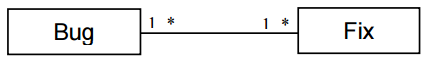
\includegraphics[scale=0.5]{media/bug-taxo-class-diag.png}
    \caption{Class diagram showing the relationship between bugs and fixed
    \label{fig:bug-taxo-diag}}
\end{figure}

\begin{figure}[h!]
  \centering
    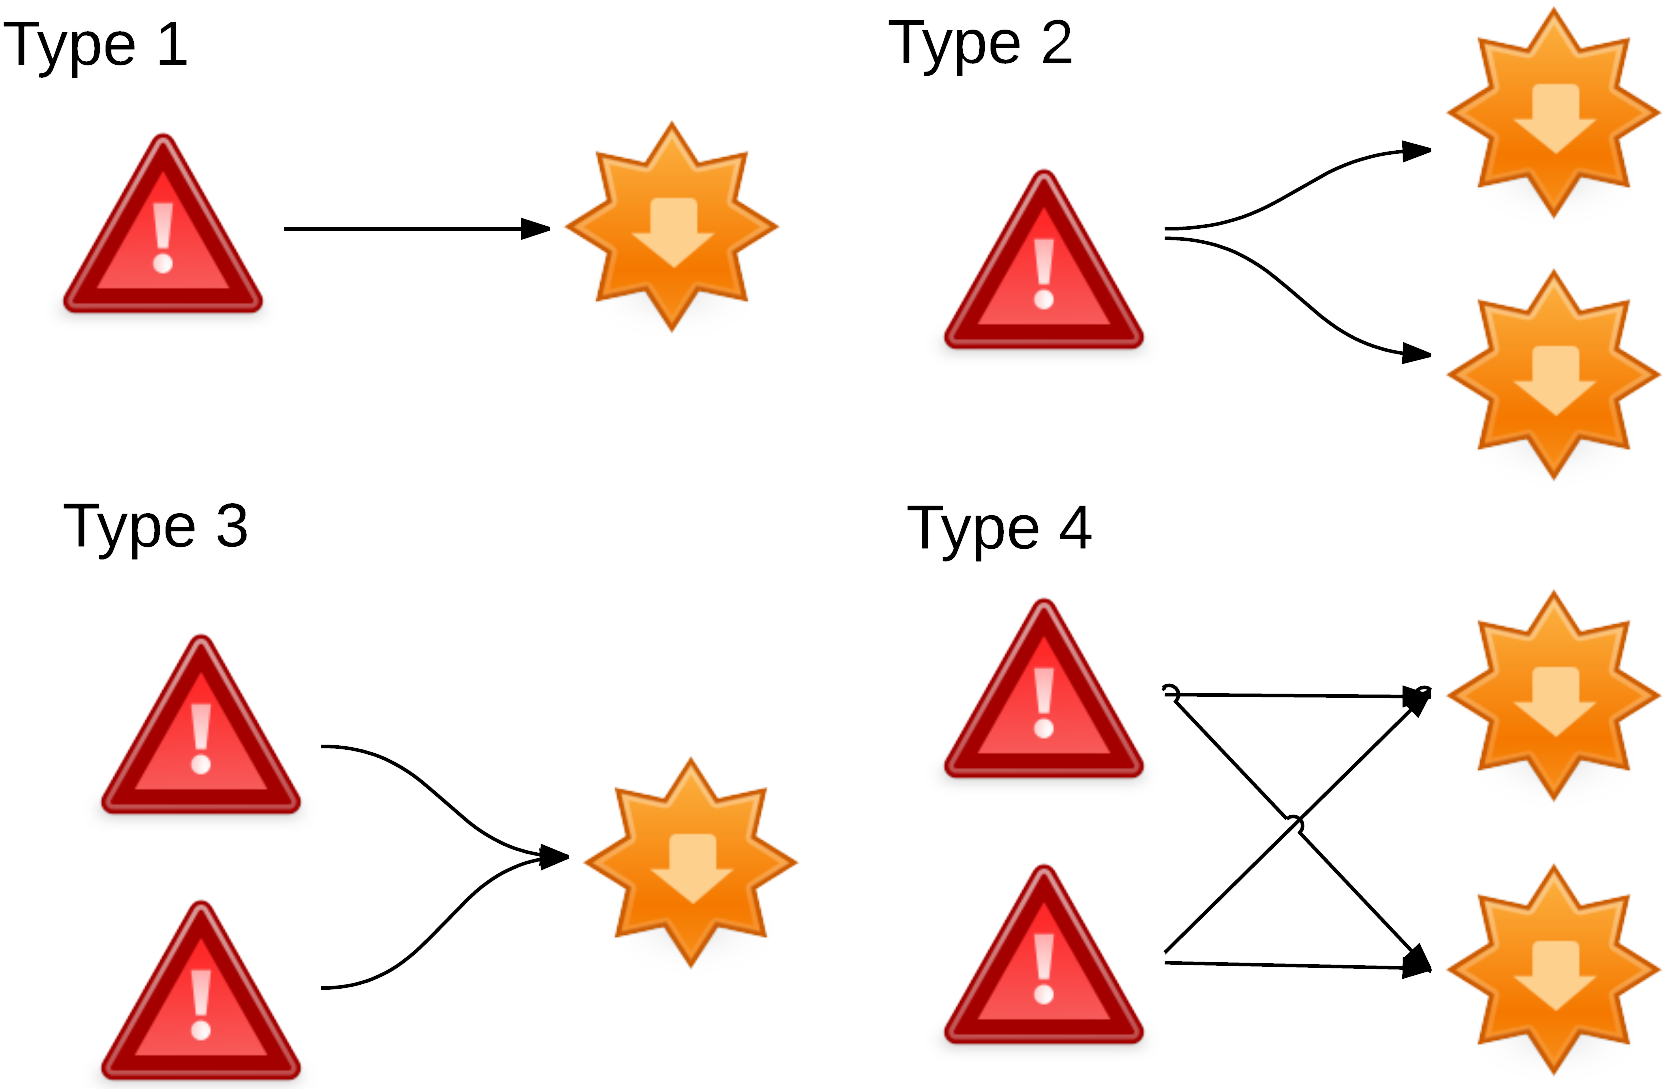
\includegraphics[scale=0.8]{media/bug-taxo.png}
    \caption{Proposed Taxonomy of Bugs
    \label{fig:bug-taxo}}
\end{figure}


The first and second types are the ones we intuitively know
about. Type 1 refers to a bug being fixed in one single location
(i.e., one file), while Type 2 refers to bugs being fixed in more
than one location. In Figure 2, only two locations are shown
for the sake of clarity, but many more locations could be
involved in the fix of a bug. Type 3 refers to multiple bugs that
are fixed in the exact same location. Type 4 is an extension of
Type 3, where multiple bugs are resolved by modifying the
same set of locations. Note that Type 3 and Type 4 bugs are
not duplicates, they may occur when different features of the
system fail due to the same root causes (faults).
We conjecture that knowing the proportions of each type
of bugs in a system may provide insight into the quality of the
system. Knowing, for example, that in a given system the
proportion of Type 2 and 4 bugs is high may be an indication
of poor system quality since many fixes are needed to address
these bugs. In addition, the existence of a high number of
Types 3 and 4 bugs calls for techniques that can effectively
find bug reports related to an incoming bug during triaging.
This is similar to the many studies that exist on detection of
duplicates (e.g., \cite{Runeson2007,Sun2010,Nguyen2012}), except that we are not looking for
duplicates but for related bugs (bugs that are due to failures of
different features of the system, caused by the same faults). To
our knowledge, there is no study that exmpirically examines
bug data with these types in mind, which is the main objective
of this section. More particularly, we are interested in the
following research questions:

\begin{itemize}
	\item RQ1: What are the proportions of different types of bugs?
	\item RQ2: How complex is each type of bugs?
	\item RQ3: How fast are these types of bugs fixed?
\end{itemize}


\section{Study Setup}

Figure \ref{fig:bug-taxo-flow} illustrates our data collection and analysis
process that we present here and discuss in more detail in the
following subsections. First, we extract the raw data from the
two bug report management systems used in this study
(Bugzilla and Jira). Second, we extract the fix to the bugs
from the source code version control system of Netbeans and
Apache (Maven and Git).

\begin{figure}[h!]
  \centering
    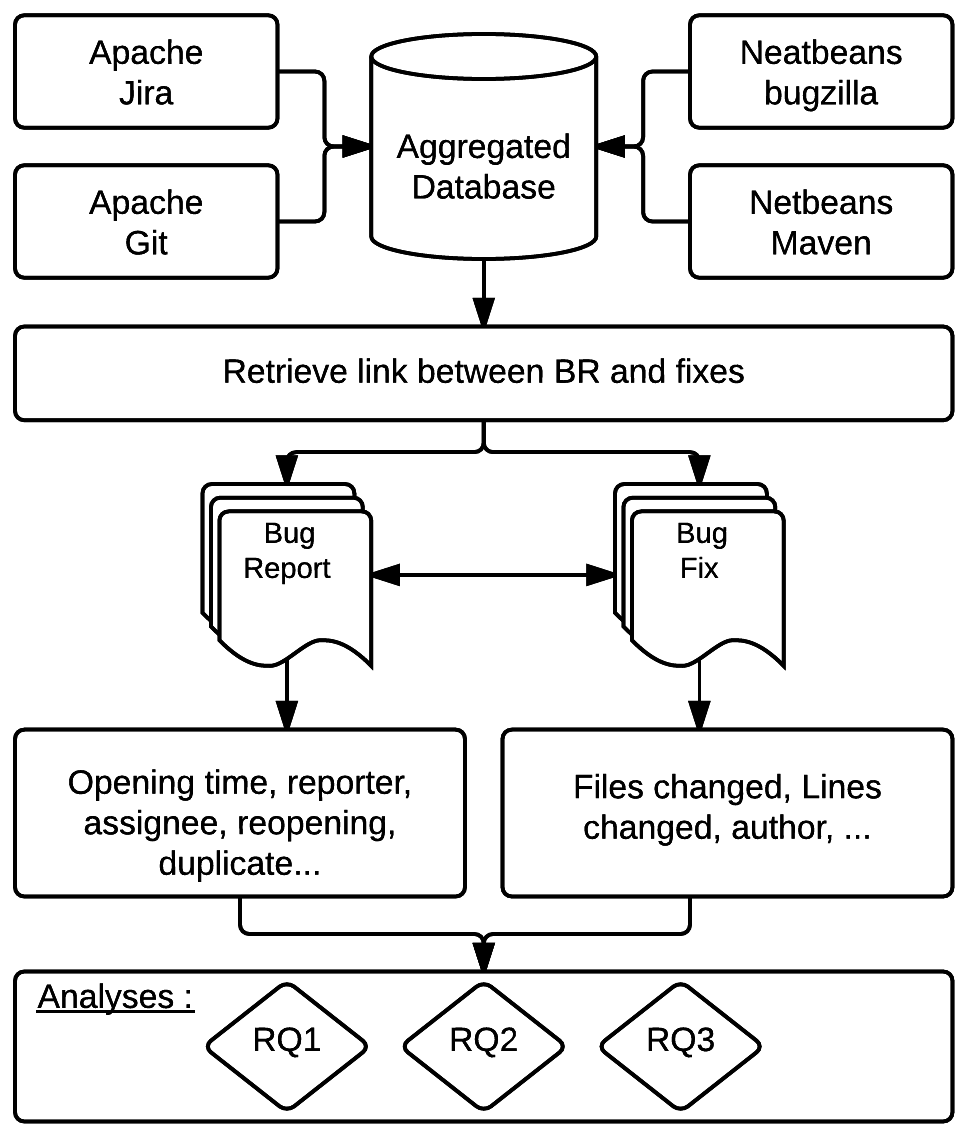
\includegraphics{media/bug-taxo-flow.png}
    \caption{Data collection and analysis process of the study
    \label{fig:bug-taxo-flow}}
\end{figure}


The extracted data is
consolidated in one database where we associate each bug
report to its fix. We mine relevant characteristics of BRs and
their fixes such as opening time, number of comments,
number of times the BR is reopened, number of changesets
for BR and the number of files changed and lines modified
for fixes or patch. Finally, we analyze these characteristics to
answer the aforementioned research questions (RQ).


\section{Study Design}

We describe the design of our study by first stating the
research questions, and then explaining the variables, and
analysis methods we used to answer these questions. We
formulate three research questions (RQs) with the ultimate
goal to improve our understanding of each bug type. We
focus, however, on Types 2 and 4. This is because these bugs
require multiple fixes. They are therefore expected to be more
complex.
The objective of the first research question is to analyze
the proportion of each type of bugs. The remaining two
questions address the complexity of the bugs and the bug
fixing duration according to the type of bugs.
1)

\subsection{RQ 1: What are the proportions of different types of bugs?}

The answer to this question provides insight into the
distribution of bugs according to their type with a focus on
Type 2 and 4 bugs. As discussed ealier, knowing, for
example, that bugs of Type 2 and 4 are the most predominant
ones suggests that we need to investigate techniques to help
detect whether an incoming bug is of Types 2 and 4 by
examining historical data. Similarly, if we can automatically
identify a bug that is related to another one that has been fixed
then we can reuse the results of reproducing the first bug in
reproducing the second one.

{\bf Hypothesis}: To answer this question, we analyze whether
Type 2 and 4 bugs are predominant in the studied systems, by
testing the null hypothesis:

\begin{itemize}
	\item $H_{01A}$ : The proportion of Types 2 and 4 does not
change significantly across the studied systems
\end{itemize}


We test this hypothesis by observing both a “global”
(across systems) and a “local” predominance (per system) of
the different types of bugs. We must observe these two
aspects to ensure that the predominance of a particular type of
bug is not circumstantial (in few given systems only) but is
also not due to some other, unknown factors (in all systems
but not in a particular system).

{\bf Variables}: We use as variables the amount of resolved/fixed
bugs of each type (1, 2, 3 and 4) that are linked to a fix
(commit). As mentioned earlier, duplicate bugs are excluded.
These are marked as resolved/duplicate in our dataset.

{\bf Analysis Method}: We answer RQ1 in two steps. The first
step is to use descriptive statistics; we compute the ratio of
Types 2 and 4 bugs and the ratio of Types 1 and 3 bugs to the
total number of bugs in the dataset. This shows the
importance of Types 2 and 4 bugs compared to Types 1 and 3
bugs.

In the second step, we compare the proportions of the
different types of bugs with respect to the system where the
bugs were found. We build the contingency table with these
two qualitative variables (the type and studied system) and
test the null hypothesis H 01A to assess whether the proportion
of a particular type of bugs is related to a specific system or
not.

We use the Pearson's chi-squared test to reject the null
hypothesis $H_{01A}$ . Pearson’s chi-squared independence test is
used to analyze the relationship between two qualitative data,
in our study the type bugs and the studied system. The results
of Pearson’s chi-squared independence test are considered
statistically significant at $\alpha$ = 0.05. If p-value $\le$ 0.05, we
reject the null hypothesis $H_{01A}$ and conclude that the
proportion of types 3 and 4 bugs is different from the
proportion of type 1 and 2 bugs for each system.

\subsection{RQ 2: How complex is each type of bugs?}

We address the relation between Types 2 and 4 bugs and
the complexity of the bugs in terms of severity, duplicate and
reopened.We analyze whether Types 2 and 4 bugs are more
complex to handle than Types 1 and 3 bugs, by testing the
null hypotheses:

\begin{itemize}
 \item  $H_{02S}$ : The severity of Types 2 and 4 bugs is not
significantly different from the severity of Types 1 and 3
 \item  $H_{02D}$ : Types 2 and 4 bugs are not significantly more
likely to get duplicated than Types 1 and 3.
 \item  $H_{02R}$ : Type 2 and 4 bugs are not significantly more
likely to get reopened than Types 1 and 3.
\end{itemize}

{\bf Variables}: We use as independent variables for the
hypotheses $H_{02S}$ , $H_{02D}$ , $H_{02R}$ the bug type (if the bug is from
Types 2 and 4 or if it is from Types 1 and 3). For $H_{02S}$  we use
the severity as dependent variable to assess the relationship
between the bug severity and the bug type. For $H_{02D}$
(respectively $H_{02R}$) we use a dummy variable duplicated
(reopened) to assess if a bug has been duplicated (reopened)
at least once or not. This will be used to assess the
relationship between the type of the bugs and the fact that the
bug is more likely to be reopened or duplicated.

{\bf Analysis Method}: For each hypothesis, we build a
contingency table with the qualitative variables type of bugs
(2 and 4 or 1and 3) and the dependent variable duplicated
(respectively reopened) and the severity variable.

We use the Pearson’s chi-squared test to reject the null
hypothesis $H_{02D}$ (respectively $H_{02R}$ ) and $H_{02S}$. The results of
Pearson’s chi-squared independence test are considered
statistically significant at $\alpha$ = 0.05. If a p-value $\le$ 0.05, we
reject the null hypothesis  $H_{02D}$ (respectively $H_{02R}$) and
conclude the fact that the bug is more likely to be duplicated
(respectively reopened) is related to the type of the bug and
we reject $H_{02S}$ and conclude that the severity level of the bug
is related to the bug type.

\subsection{RQ 3 : How fast are these types of bugs fixed ?}

In this question, we study the relation between the
different types of bugs and the fixing time. We are interested
in evaluating whether developers take more time to fix Types
2 and 4 bugs than Type 1 and 3, by testing the null hypothesis:

\begin{itemize}
	\item $H_{03}$ : There is no statistically-significant difference
between the duration of fixing periods for Types 2 and
4 bugs and that of Types 1 and 3 bugs.
\end{itemize}


{\bf Variables}: To compare the bug fixing time with respect to
their type, we use as independent variable the type Ti of a
bug Bi, to distinguish between Types 1 and 3 bugs and Types
2 and 4 bugs. We consider as dependent variable the fixing
time, FTi, of the bug Bi. We compute the fixing time FTi of a
bug Bi. The fixing time FTi is the time between when the bug
is submitted to when it is closed/fixed.

{\bf Analysis Method}: We compute the (non-parametric) Mann-
Whitney test to compare the BR fixing time with respect to
the BR type and analyze whether the difference in the average
fixing time is statistically significant. We use the Mann-
Whitney test because, as a non-parametric test, it does not
make any assumption on the underlying distributions. We
analyze the results of the test to assess the null hypothesis
$H_{03}$ . The result is considered as statistically significant at $\alpha$ =
0.05. Therefore, if p-value $\le$ 0.05, we reject the null
hypothesis H 03 and conclude that the average fixing time of
Types 1 and 3 bugs is significantly different from the average
fixing time of Types 2 and 4 bugs.

\section{Study result and discussion}

In this section, we report on the results of the analyses we
performed to answer our research questions. We then dedicate
a section to discussing the results.

\subsection{RQ 1 : What are the proportions of different types of
bugs?}

Figure \ref{fig:bug-taxo-rq1} shows the percentage of the different types of
bugs. As shown in the figure, we found that 65\% of the bugs
are from Types 2 and 4. This shows the predominance of this
type of bugs in all the studied systems. Figure 5 shows the
repartition per dataset. We can see that Netbeans and Apache
have 66\% and 64\% bugs of Type 1and 3, respectively. To
ensure that this observation is not related to a particular
system, we perform Pearson’s chi-squared test across the
studied systems. Table \ref{tab:bug-taxo-rq1} shows the contingency table for the
studied systems and the result of Pearson’s chi-squared test.
The results show that there is statistically significant
difference between the proportions of the different types of
bugs.

\begin{table}[h!]
\centering
\begin{tabular}{c|c|c|c}
{System} & {Type 1 and 3} & {Type 2 and 4} & {Pearson’s chisquared p-value}        \\  \hline \hline
Apache       & 4910               & 8626               & \multirow{2}{*}{p-value \textless 0,0001} \\ \cline{1-3}
Netbeans     & 9050               & 17586              & \\ \hline \hline
\end{tabular}
\caption{Contingency table and Pearson's chi-squared tests\label{tab:bug-taxo-rq1}}
\end{table}

\begin{figure}[h!]
  \centering
    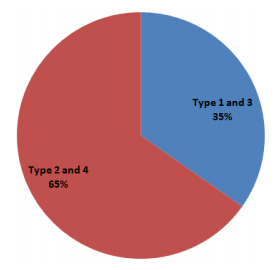
\includegraphics[scale=0.7]{media/bug-taxo-rq1.png}
    \caption{Proportions of different types of bugs
    \label{fig:bug-taxo-rq1}}
\end{figure}

Table \ref{tab:bug-taxo-rq1-prop} shows the number of bugs for each type of bugs
and the percentage of each type of bugs. We can see that
Types 3 and 4 bugs represent 28.33\% and 61.21\% of the total
of bugs, respectively. Types 1 and 2 represent only 6.78\% and
3.74\%. Together, Types 3 and 4 bugs represent almost 90\%
of the total number of bugs linked to a commit.

\begin{table}[h!]
\centering

\begin{tabular}{c|c|c|c|c|c}
Datasets                  & T1        & T2       & T3        & T4        & Total                  \\ \hline \hline
\multirow{2}{*}{Netbeans} & 776       & 240      & 8372      & 17366     & \multirow{2}{*}{26754} \\
                          & (2.90\%)  & (0.90\%) & (31.29\%) & (64.91\%) &                        \\ \hline
Apache                    & 1968      & 1248     & 3101      & 7422      & \multirow{2}{*}{13739} \\
                          & (14.32\%) & (9.08\%) & (22.57\%) & (54.02\%) &                        \\ \hline
\multirow{2}{*}{Total}    & 2744      & 1488     & 11473     & 24788     & \multirow{2}{*}{40493} \\
                          & (6.78\%)  & (3.74\%) & (28.33\%) & (61.21\%) & \\ \hline \hline
\end{tabular}
\caption{Proportion of bug types in amount and percentage}
\label{tab:bug-taxo-rq1-prop}
\end{table}


\noindent\fbox{%
    \parbox{\textwidth}{%
      We can thus reject the null hypothesis $H_{01A}$ and
conclude that there is a predominance of Types 2 and
4 bugs in all studied systems and this observation is
not related to a specific system.
    }%
}

\subsection{RQ 2 : How complex is each type of bugs?}

Figure \ref{fig:bug-taxo-rq2-prop-apache} and \ref{fig:bug-taxo-rq2-prop-netbeans} show the proportion of each bug type with
respect to their severity for each dataset. Table V shows the
proportion of each bug type with repect to their severity and
dataset. For Netbeans, the bugs we examined in our dataset
are either labeled as Blocker or Normal (despite the fact that
Netbeans uses Bugzilla that supports all the severity levels
presented in the previous section).

\begin{figure}[h!]
  \centering
    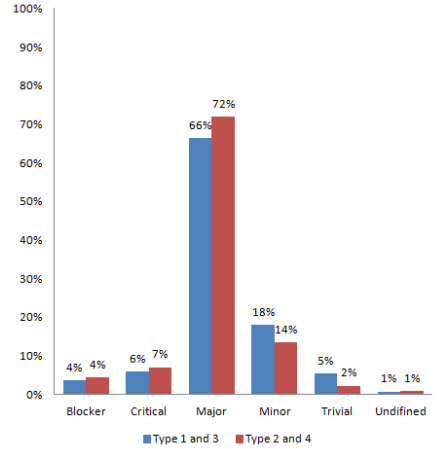
\includegraphics[scale=0.6]{media/bug-taxo-rq2-prop-apache.png}
    \caption{Proportions of Types 1 and 3 versus Types 2 and 4 with respct to their severity in the Apache dataset.
    \label{fig:bug-taxo-rq2-prop-apache}}
\end{figure}

\begin{figure}[h!]
  \centering
    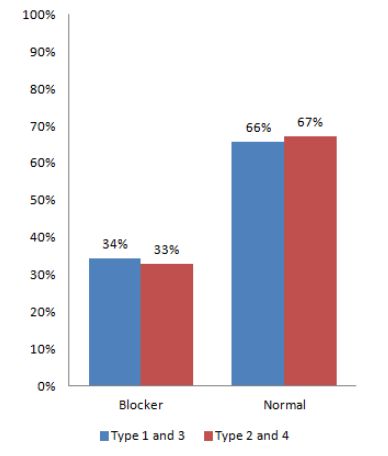
\includegraphics[scale=0.6]{media/bug-taxo-rq2-prop-netbeans.png}
    \caption{Proportions of Types 1 and 3 versus Types 2 and 4 with respct to their severity in the Netbeans dataset.
    \label{fig:bug-taxo-rq2-prop-netbeans}}
\end{figure}

For the Apache dataset, the severity levels range from
Blocker to Trivial as shown in Figure \ref{fig:bug-taxo-rq2-prop-apache}. Figure \ref{fig:bug-taxo-rq2-prop-netbeans} shows that
in Netbeans around 67\% of Types 2 and 4 bugs are normal.
The same holds for Types 1 and 3 bugs (66\% are considered
of normal severity). This indicates that most Types 2 and 4
bugs and Types 1 and 3 bugs are not critical in the Netbeans
dataset. For the Apache dataset, the results indicate that the
majority of the bugs are considered of major severity (66\%
for Types 1 and 3 and 72\% for Types 2 and 4). It is
challenging to understand the discrepancy between the two
datasets partly because of the way the severity is assigned to
BRs.

Table \ref{tab:bug-taxo-rq2-chi} shows the result of the Pearson chi-squared tests
for the $H_{02S}$, $H_{02D}$ and $H_{02R}$ hypotheses.

\begin{table}[h!]
\centering
\begin{tabular}{c|c|c}
System                    & Factor     & \begin{tabular}[c]{@{}c@{}}Pearson’s chisquared\\ p-value\end{tabular} \\ \hline \hline
\multirow{3}{*}{Apache}   & Severity   & p-value \textless 0.005                                                \\
                          & Reopened   & p-value \textless 0.005                                                \\
                          & Duplicated & p-value \textless 0.005                                                \\ \hline \hline
\multirow{3}{*}{Netbeans} & Severity   & p-value \textless 0.005                                                \\
                          & Reopened   & p-value \textless 0.005                                                \\
                          & Duplicated & p-value \textless 0.005  \\  \hline \hline
\end{tabular}

\caption{Pearson's chi squared p-values for the severity, the reopen and the duplicate factor with respect to a dataset}
\label{tab:bug-taxo-rq2-chi}
\end{table}

\noindent\fbox{%
    \parbox{\textwidth}{%
      According to the results of the test (p-value < 0.005),
we reject the null hypothesis $H_{02S}$ and conclude that
there is a significant difference between the severity of
Types 1 and 3 bugs and the severity of Types 2 and 4
bugs.
    }%
}

\begin{table}[h!]
\centering
\begin{tabular}{c|c|c|c|c}
Severity                  & T1      & T2      & T3      & T4      \\
\hline \hline
\multicolumn{5}{c}{Netbeans}                                      \\ \hline
\multirow{2}{*}{Blocker}  & 340     & 109     & 2850    & 5687    \\
                          & 43.81\% & 45.42\% & 34.04\% & 32.75\% \\ \hline
\multirow{2}{*}{Normal}   & 436     & 131     & 5522    & 11678   \\
                          & 56.19\% & 54.58\% & 65.96\% & 67.25\% \\
                          \hline
\multirow{2}{*}{Total}    & 776     & 240     & 8372    & 17365   \\
                          & 100\%   & 100\%   & 100\%   & 100\%   \\
\hline \hline
\multicolumn{5}{c}{Apache}                                        \\ \hline
\multirow{2}{*}{Blocker}  & 68      & 53      & 115     & 329     \\
                          & 3.46\%  & 4.25\%  & 3.71\%  & 4.43\%  \\
                          \hline
\multirow{2}{*}{Critical} & 84      & 44      & 213     & 565     \\
                          & 4.27\%  & 3.53\%  & 6.87\%  & 7.61\%  \\
                          \hline
\multirow{2}{*}{Major}    & 1245    & 811     & 2096    & 5427    \\
                          & 63.26\% & 64.98\% & 67.59\% & 73.12\% \\
                          \hline
\multirow{2}{*}{Minor}    & 408     & 276     & 501     & 899     \\
                          & 20.73\% & 22.12\% & 16.16\% & 12.11\% \\
                          \hline
\multirow{2}{*}{Trivial}  & 113     & 31      & 159     & 161     \\
                          & 5.74\%  & 2.48\%  & 5.13\%  & 2.17\%  \\
                          \hline
\multirow{2}{*}{Total}    & 1918    & 1215    & 3084    & 7381    \\
                          & 100\%   & 100\%   & 100\%   & 100\%  \\
\hline \hline
\end{tabular}
\caption{Proportion of each bug type with respect to severity.}
\label{tab:bug-taxo-rq2-severity}
\end{table}

Table \ref{tab:bug-taxo-rq2-dup} shows the occurrences of duplicate and reopened
bugs with respect to their bug type in each dataset. In
Netbeans, the proportion of Type 1 bugs that are marked as
source of duplicate is 6.06\%, 4.59\% for Type 2 bugs, 5.09\%
for Type 3 bugs and 5.87\% for Type 4 bugs with a total of
1503 bugs over 26754 (5.62\%). In Apache, the proportion of
Type 1 bug marked a source of a duplicate is 2.59\% and
2.24\%, 1.61\% and 2.91\% for Types 2, 3 and 4, respectively.

\begin{table}[h!]
\centering
\begin{tabular}{c|c|c|c|c|c}
Type                   & T1     & T2     & T3     & T4     & Total  \\ \hline \hline
\multicolumn{6}{c}{Netbeans}                                      \\ \hline \hline
\multirow{2}{*}{Dup.}  & 6.06\% & 4.59\% & 5.09\% & 5.87\% & 5.62\% \\
                       & (47)   & (11)   & (426)  & (1019) & (1503) \\ \hline
\multirow{2}{*}{Reop.} & 4.38\% & 7.08\% & 4.81\% & 7.09\% & 6.30\% \\
                       & (34)   & (17)   & (403)  & (1231) & (1685) \\ \hline
\multicolumn{6}{c}{Apache}                                        \\ \hline \hline
\multirow{2}{*}{Dup}   & 2.59\% & 2.24\% & 1.61\% & 2.91\% & 2.51\% \\ \
                       & (51)   & (28)   & (50)   & (216)  & (345)  \\ \hline
\multirow{2}{*}{Reop}  & 5.59\% & 6.49\% & 3.10\% & 6.90\% & 5.82\% \\
                       & (110)  & (81)   & (96)   & (512)  & (799)  \\ \hline
\multicolumn{6}{c}{Total}                                         \\ \hline \hline
\multirow{2}{*}{Dup}   & 3.57\% & 2.62\% & 4.15\% & 4.98\% & 4.56\% \\
                       & (98)   & (39)   & (476)  & (1235) & (1848) \\ \hline
\multirow{2}{*}{Reop}  & 5.25\% & 6.59\% & 4.35\% & 7.03\% & 6.13\% \\
                       & (144)  & (98)   & (499)  & (1743) & (2484) \\ \hline
\end{tabular}
\caption{Percentage and occurences of bugs duplicated by other bufs and reopenned with respect to their bug type and dataset.}
\label{tab:bug-taxo-rq2-dup}
\end{table}

Second, we analyze the reopened bugs to see the link
between the reopening and the type of bugs. We perform
Pearson’s chi-squared test to reject the null hypothesis $H_{02R}$.

\noindent\fbox{%
    \parbox{\textwidth}{%
      According to the results of the test (p-value <
0.005), we reject the null hypothesis $H_{02R}$ and
conclude that there is a significant relationship
between the reopening of a bug and its type.
    }%
}

Third, we analyze the duplicated bugs to see if there is a
link between the bug type and the fact duplication. We
perform Pearson’s chi-squared test to reject the null
hypothesis $H_{02D}$.

\noindent\fbox{%
    \parbox{\textwidth}{%
      According to the results of the test (p-value <
0.005), we reject the null hypothesis $H_{02D}$ and
conclude that there is a significant relationship
between the duplication of a bug and its type.
    }%
}

\subsection{RQ 3 : How fast are these types of bugs fixed ?}

Figure \ref{fig:bug-taxo-rq3} shows the fixing time for Types 1 and 3 versus
Types 2 and 4 for Netbeans and the Apache Software
Foundation. In Netbeans, 98.96 and 137.05 days are required
to fix Types 1 and 3 and Types 2 and 4, respectively. In
Apache, 55.76 and 85.48 days are required to fix Types 1 and
3 and Types 2 and 4, respectively.


\begin{figure}[h!]
  \centering
    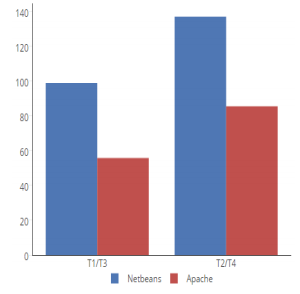
\includegraphics[scale=0.8]{media/bug-taxo-rq3.png}
    \caption{Fixing time of Types 1 and 3 versus fixing time of Types 2 and 4.
    \label{fig:bug-taxo-rq3}}
\end{figure}

Table \ref{tab:bug-taxo-rq3} shows the average fixing time of bugs with respect
to their bug type in each dataset.

\begin{table}[h!]
\centering
\begin{tabular}{c|c|c|c|c|c}
Dataset  & T1    & T2     & T3     & T4     & Average \\ \hline \hline
Netbeans & 97.66 & 117.42 & 100.26 & 156.67 & 118.00  \\ \hline
Apache   & 73.48 & 118.12 & 38.04  & 52.83  & 70.62   \\ \hline
Total    & 85.57 & 117.77 & 69.15  & 104.75 & 94.31  \\ \hline \hline
\end{tabular}
\caption{Average fixing time with respect to bug type
    \label{tab:bug-taxo-rq3}}
\end{table}

We analyze the difference in the fixing time of bugs with
respect to their bug type by conducting a Mann-Whitney test
to assess $H03$.The results show that the difference between
the fixing time of Types 2 and 4 and Types 1 and 3 is
statistically significant (p-value < 0,005).

\noindent\fbox{%
    \parbox{\textwidth}{%
      Therefore, we can reject the null hypothesis $H03$ and
conclude that the fixing of Types 2 and 4 bugs takes
more time than the fixing of Types 1 and 3 bugs.
    }%
}

\subsubsection{Dicussion}

{\bf Repartition of bug types}: One important finding of this
study is that there is significantly more Types 2 and 4 bugs
than Types 1 and 3 in all studied systems. Moreover, this
observation is not system-specific. The traditional one-bug/
one-fault way of thinking about bugs only accounts for 35\%
of the bugs. We believe that, recent triaging algorithms
\cite{Jalbert2008,Jeong2009,Khomh2011a,Tamrawi2011a} can benefit from these findings by developing
techniques that can detect Type 2 and 4 bugs. This would
result in better performance in terms of reducing the cost,
time and efforts required by the developers in the bug fixing
process.

{\bf Severity of bugs}: We discussed the severity and the
complexity of a bug in terms of its likelihood to be reopened
or marked as duplicate (RQ2). Although clear guidelines exist
on how to assign the severity of a bug, it remains a manual
process done by the bug reporter. In addition, previous
studies, notably those by Khomh et al. \cite{Khomh2011a}, showed that severity is not a consistent/trustworthy characteristic of a BR,
which lead to he emergence of studies for predicting the
severity of bugs (e.g., \cite{Lamkanfi2010,Lamkanfi2011,Tian2012}). Nevertheless, we
discovered that there is a significant difference between the
severities of Types 1 and 3 compared to Types 2 and 4.

{\bf Complexity of bugs}: At the complexity level, we use the
number of times a bug is reopened as a measure of
complexity. Indeed, if a developer is confident enough in
his/her fix to close the bug and that the bug gets reopened it
means that the developer missed some dependencies of the
said bug or did not foresee the consequences of the fix.
We found that there is a significant relationship between
the number of reopenings and type of a bug. In other words,
there is a significant relationship between the complexity and
the type of a given bug. In our datasets, Types 1 and 3 bugs
are reopened in 1.88\% of the cases, while Types 2 and 4 are
reopened in 5.73\%. Assuming that the reopening is a
representative metric for the complexity of bug, Types 2 and
4 are three times more complex than Types 1 and 3. Finally, if
we consider multiple reopenings, Types 2 and 4 account for
almost 80\% of the bugs that reopened more than once and
more than 96\% of the bug opened more than twice.
While current approaches aiming to predict which bug
will be reopen use the amount of modified files \cite{Shihab2010,Zimmermann2012,Lo2013}, we
believe that they can be improved by taking into account the type of a the bug. For example, if we can detect that an
incoming bug if of Type 2 or 4 then it is more likely to
reopened than a bug of Type 1 or 3. Similarly, approaches
aiming to predict the files in which a given bug should be
fixed could be categorized and improved by knowking the
bug type in advance \cite{Zhou2012,Kim2013a}.

{\bf Impact of a bug}: To measure the impact of bugs in end-users
and developers, we use the number of times a bug is
duplicated. This is because if a bug has many duplicates, it
means that a large number of users have experienced and a
large number of developers are blocked the failure.
We found that there is a significant relationship between
the bug type and the fact that it gets duplicated. Types 1 and 3
bugs are duplicated in 1.41\% of the cases while Types 2 and 4
are duplicated in 3.14\%. Assuming that the amount of
duplication is an accurate metric for the impact of bug, Types
2 and 4 have more than two times bigger impact than Types 1
and 3. Similarly to reopening, if we consider multiple
duplication, Types 2 and 4 account for 75\% of the bugs that
get duplicated more than once and more than 80\% of the bugs
that get duplicated more than twice.
We believe that approaches targeting the identification of
duplicates \cite{Bettenburg2008a,Jalbert2008,Sun2010,Tian2012a}  could leverage this taxonomy to
achieve even better performances in terms of recall and
precision.

{\bf Fixing time}: Our third research question aimed to determine
if the type of a bug impacts its fixing time. Not only we found
that the type of a bug does significantly impact its fixing time,
but we also found that, in average Types 2 and 4, stay open
111.26 days while Types 1 and 3 last for 77.36 days. Types 2
and 4 are 1.4 time longer to fix than Types 1 and 3.We
therefore believe that, approaches aiming to predict the fixing
time of a bug (e.g., \cite{Panjer2007,Bhattacharya2011,Zhang2013}) can highly benefit from
accurately predicting the type of a bug and thereforebetter
plan the required man-power to fix the bug.
In summary, Types 2 and 4 account for 65\% of the bugs
and they are more complex, have a bigger impact and take
longer to be fixed than Types 1 and 3 while being equivalent
in terms of severity.

Our taxonomy aimed to analyse: (1) the
proportion of each type of bugs; (2) the complexity of each
type in terms of severity, reopening and duplication; (3) the
required time to fix a bug depending on its type. The key
findings are:
\begin{itemize}
  \item Types 2 and 4 account for 65\% of the bugs.
  \item Types 2 and 4 have a similar severity compared to
Types 1 and 3.
  \item Types 2 and 4 are more complex (reopening) and have
a bigger impact (duplicate) than Types 1 and 3.
  \item It takes more time to fix Types 2 and 4 than Types 1
and 3.
\end{itemize}

Our taxonomy and results can be built upon in order to classify
past and new researches in several active areas such as bug
reproduction and triaging, prediction of reopening,
duplication, severity, files to fix and fixing time. Moreover, if
one could predict the type of a bug at submission time, all
these areas could be improved.

%!TEX root = ../research_proposal.tex

With the goal to support the research towards analyzing relationships between bugs and their fixes we constructed a dataset of 380 projects, more than 100,000 resolved/fixed and with 60,000 changesets that were involved in fixing them from Netbeans and The Apache Software foundation's software that is (1) searchable in natural language at https://bumper-app.com, (2) contains clear relationships between the bug report and the code involved to fix it, (3) supports complex queries such as parent-child relationships, unions or disjunctions and (4) provide easy exports in json, csv and xml format.

In what follows, we will present the projects we selected. Then, we present the features related to the bugs and their fixes we integrate in BUMPER (BUg Metarepository for dEvelopers and Researchers) and how we construct our dataset. Then, we present the API, based on Apache Solr \cite{Nayrolles2014b}, which allows the NLP search with practical examples before providing research opportunities based on our dataset.


However, to the best of our knowledge, no attempt has been made towards building a unified and online dataset where all the information related to a bug, or a fix can be easily accessed by researchers and engineers.

\section{Data collection}

Figure \ref{fig:bumper-approach} illustrates our data collection and analysis process that we present here and discuss in more detail in the following subsections. First, we extract the raw data from the two bug report management systems used in this study (Bugzilla\footnote{https://netbeans.org/bugzilla/} and Jira\footnote{https://issues.apache.org/jira/issues/?jql=}). The extracted data is consolidated in one database called BUMPER where we associate each bug report with its fix. The fixes are mined from different type of source versioning system. Indeed, Netbeans is based on mercurial\footnote{ http://mercurial.selenic.com/} while we used the git\footnote{http://git-scm.com/} mirrors\footnote{https://github.com/apache} for the Apache Foundation software.

\begin{figure}[h!]
  \centering
    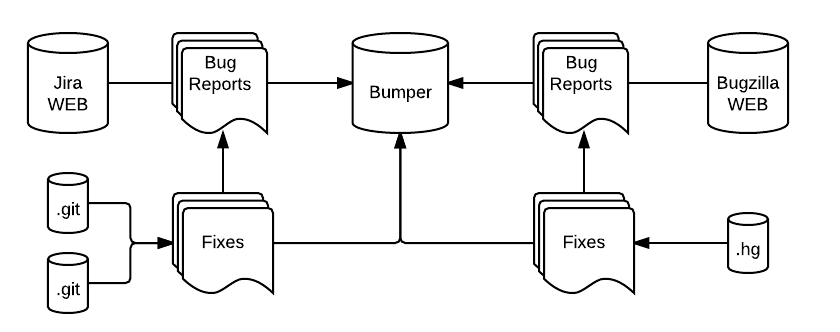
\includegraphics{media/bumper-approach.png}
    \caption{Overview of the bumper database construction.
    \label{fig:bumper-approach}}
\end{figure}

We used the same datasets presented earlier in Table \ref{table:datasets}.
We choose to use the same ones as these two datasets because they exposed a great diversity in programming languages, teams, localization, utility and maturity. Moreover, the used different tools, i.e. Bugzilla, JIRA, Git and Mercurial, and therefore, BUMPER is ready to host any other datasets that used any composition of these tools.

\section{Architecture}

{\tt BUMPER} rely on a highly scalable architecture composed of two distinct servers as depicted in Figure \ref{fig:bumper-arch}. The first server, on the left, handles the web requests and runs three distinct components:

\begin{itemize}
	\item Pound is a lightweight open source reverse proxy program and application firewall.
	It is also served us to decode  to request to http. Translating an  request to http and then, use this HTTP request instead of the  one allow us to save the http's decryption time required at each step.
	Pound also acts as a load-balancing service for the lower levels.
	\item Translated requests are then handled to Varnish. Varnish is an HTTP accelerator designed for content-heavy and dynamic websites. What it does is caching request that come in and serve the answer from the cache is the cache is still valid.
	\item NginX (pronounced engine-x) is a web-server that has been developed with a particular focus on high concurrency, high performances and low memory usage.
\end{itemize}

On the second server, that concretely handles our data, we have the following items:

\begin{itemize}
	\item Pound. Once again, we use pound here, for the exact same reasons.
	\item SolrCloud is the scalable version of Apache Solr where the data can be separated into shards (e.g chunk of manageable size). Each shard can be hosted on a different server, but it's still indexed in a central repository. Hence, we can guarantee a low query time while exponentially increasing the data.
	\item Lucene is the full text search engine powering Solr. Each Solr server has its own embedded engine.
\end{itemize}

\begin{figure}[h!]
  \centering
    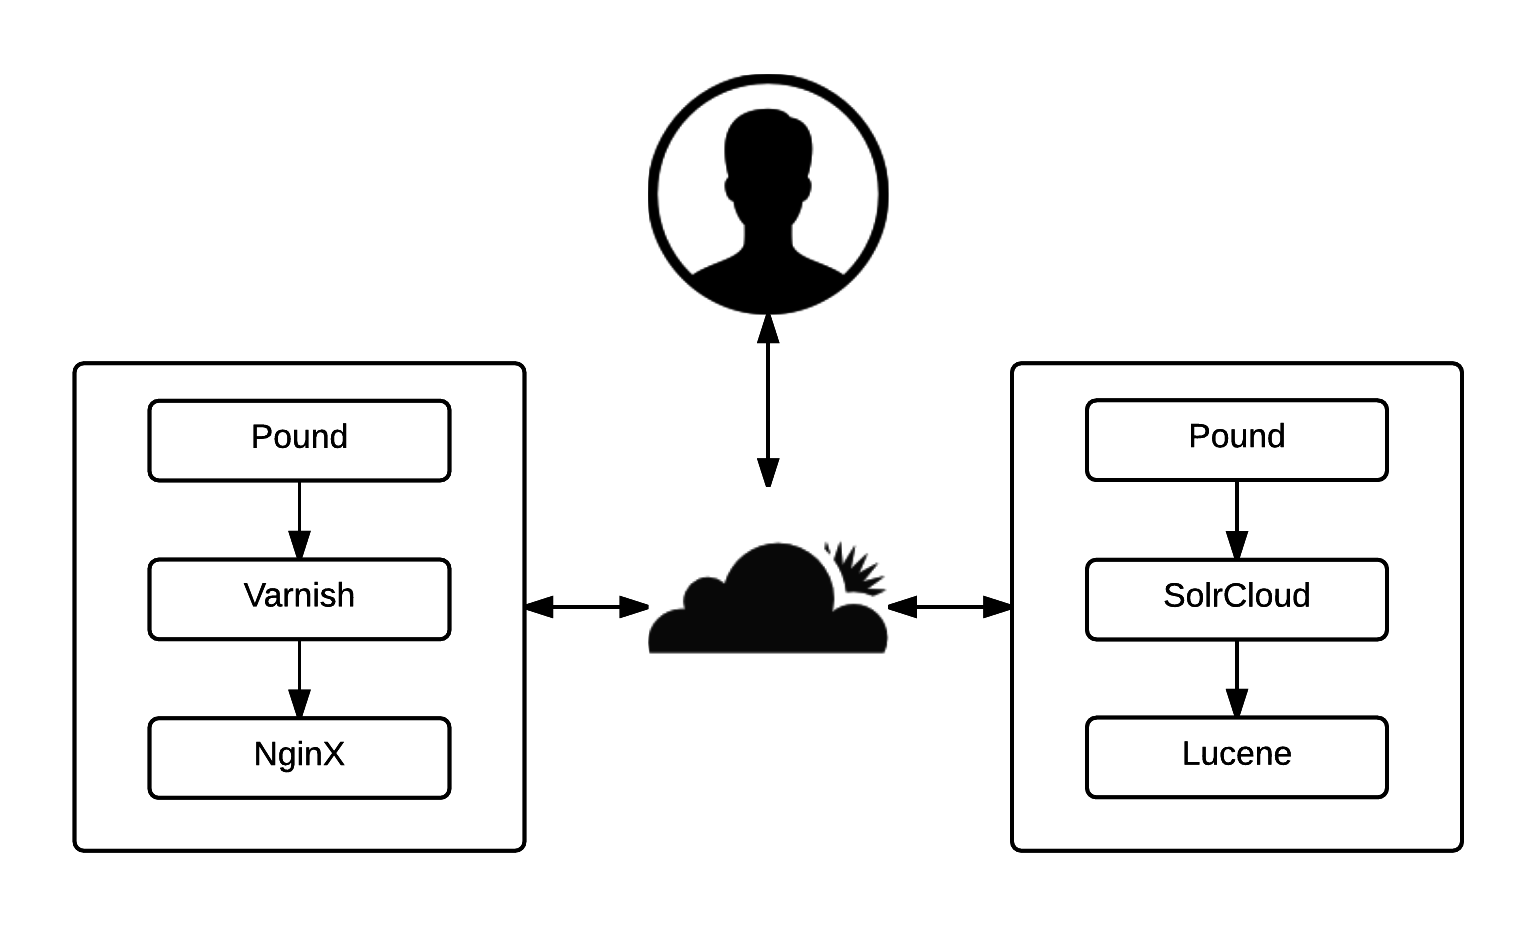
\includegraphics{media/bumper-arch.png}
    \caption{Overview of the bumper architecture.
    \label{fig:bumper-arch}}
\end{figure}

Request from users to the servers and the communication between our servers are going through the CloudFlare network.
CloudFlare acts as a content delivery network sitting between the users and the webserver.
They also provide an extra level of caching and security.

To give the reader a glimpse about the performances that this unusual architecture can yield; we are able to request and display the result of a specific request in less than 100 ms while our two servers are, in fact, two virtual machines sharing an AMD Opteron (tm) Processor 6386 SE (1 core @ 2,000 MHz) and 1 GB of RAM.

\section{UML Metamodel}

Figure \ref{fig:bumper-approach} presents the simplified {\tt BUMPER} metamodel that we designed according to our bug taxonomy presented in section \ref{fig:bug-taxo} and according to our future needs for {\tt JCHARMING}, {\tt RESSEMBLE} and {\tt BIANCA}.

\begin{figure}[h!]
  \centering
    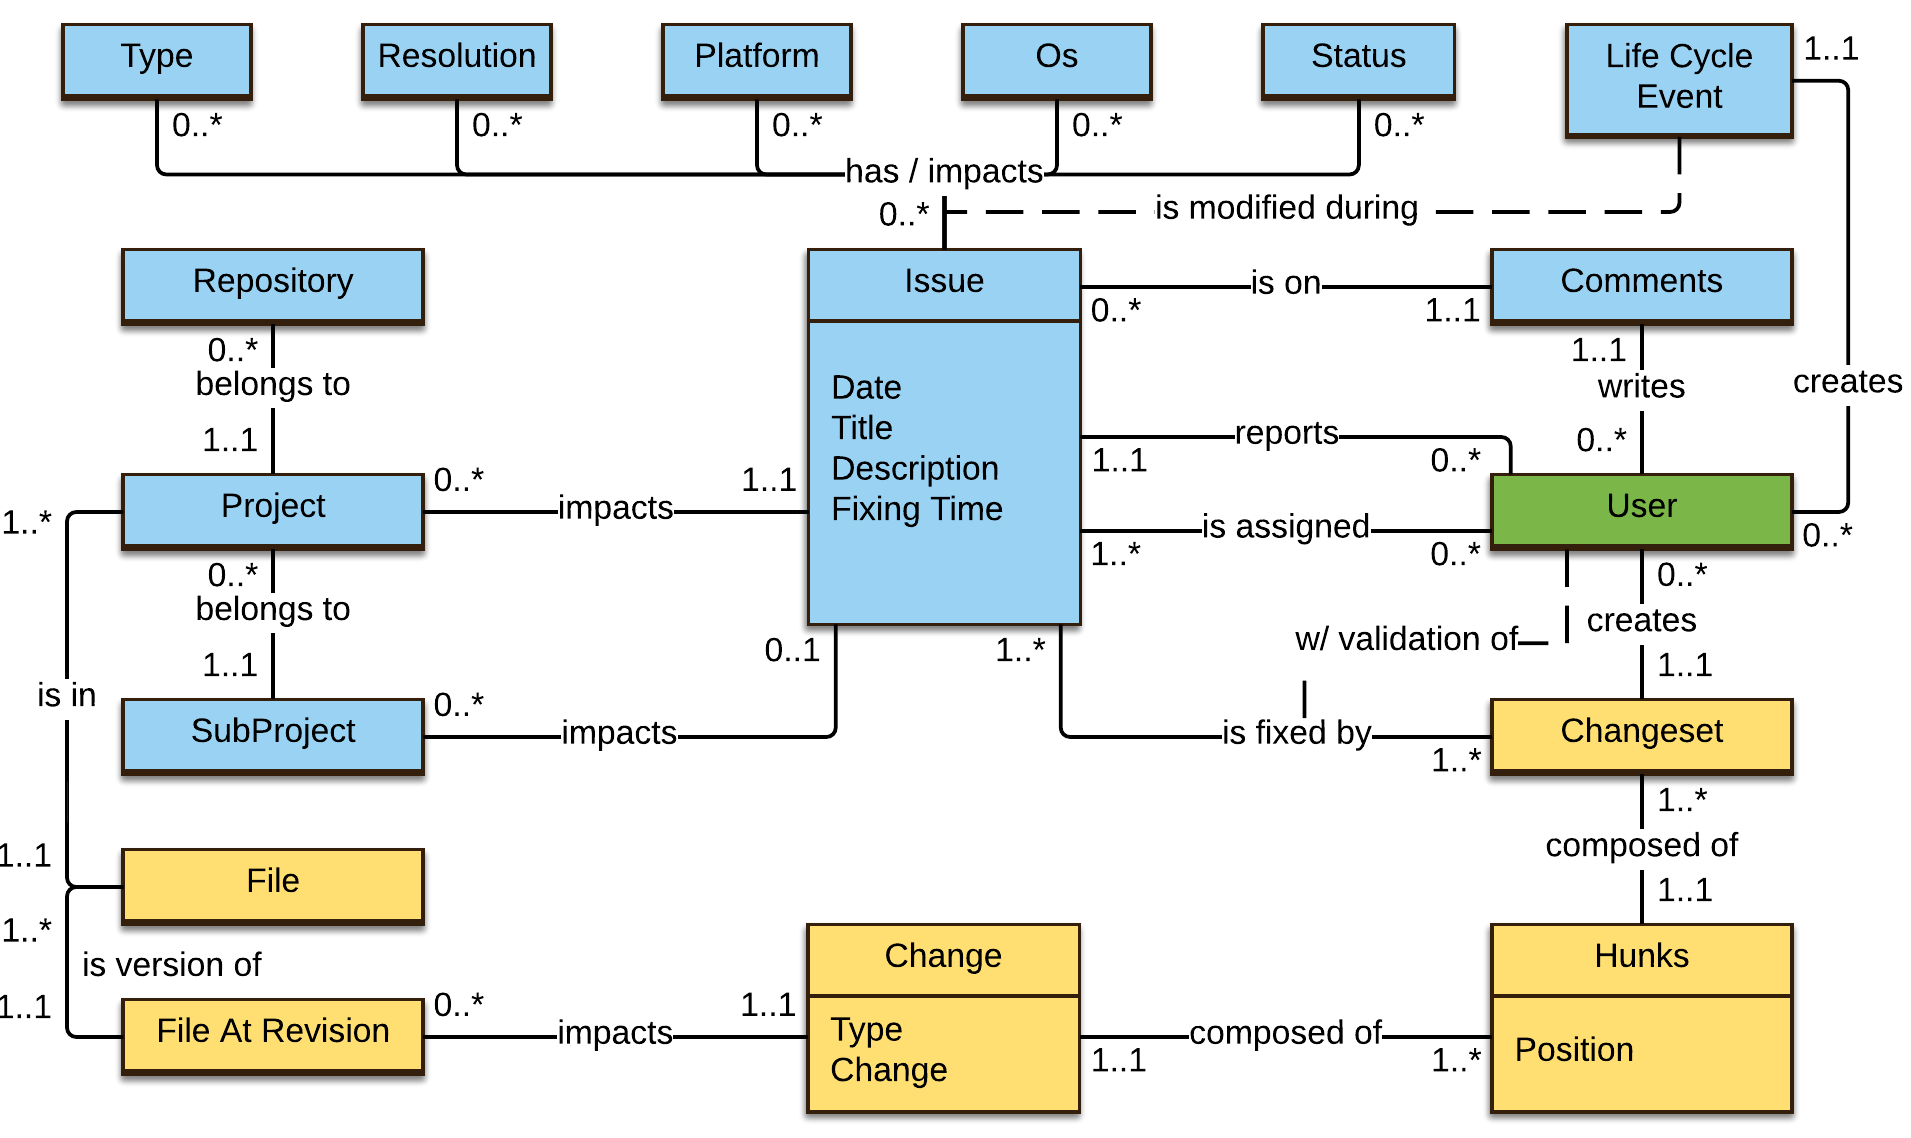
\includegraphics{media/bumper-model.png}
    \caption{Overview of the bumper meta-model.
    \label{fig:bumper-approach} }
\end{figure}


An {\it issue} ({\it task}) is characterized by a {\it date}, {\it title}, {\it description}, and a {\it fixing time}. They are reported (created) by and assigned to {\it users}.
Also, {\it issues} ({\it tasks}) belong to {\it project} that are in {\it repository} and might be composed of {\it sub-projects}.
{\it Users} can modify an {\it issue} ({\it task})  during {\it life cycle events} which impact the {\it type}, the {\it resolution}, the {\it platform}, the {\it OS} and the {\it status}. {\it Issues} ({\it tasks}) are resolved (implemented) by {\it changeset} that are composed of {\it hunks}. {\it Hunks} contain the actual changes to a {\it file} at a given revision, which are versions of the {\it file} entity that belongs to a {\it Project}.


\section{Features}

In this section, we present the features of bug report and their fixes in details.

\subsection{Bug Report}

A bug report is characterized by the following features:


\begin{itemize}

\item ID: unique string id of the form bug\_dataset\_project\_bug\_id
\item Dataset: the dataset of which the bug is extracted from.
\item Type: The type help us to distinguish different type of entities in BUMPER, i.e the bugs, changesets and hunks. For bug report, the type is always set to BUG
\item Date: The date at which the bug report has been submitted.
\item Title: The title of the bug report.
\item Project: The project that this bug affects.
\item Sub\_project: The sub-project that this bug affects.
\item Full\_name\_project: The combination of the project and the sub-project.
\item Version: the version of the project that this bug affects
\item Impacted\_platform: the platform that this bug affects
\item Impacted\_os: the operating system that this bug affects
\item Bug\_status: The status of the bug. As in bumper, our main concern is on the relationship between of fix and a bug, we only have RESOLVED bugs
\item Resolution: How the bug was resolved. Once again, as we are interested in investigating the fixes and the bugs, we only have FIXED bugs.
\item Reporter\_pseudo: the pseudonym of the person who report the bug.
\item Reporter\_name: the name of the person who reported the bug
\item Assigned\_to\_pseudo: the pseudonym of the person who have \item been assigned to fix this bug
\item Assigned\_to\_name: the name of the person who have been assigned to fix this bug
\item Bug\_severity: the severity of a bug
\item Description: the description of the bug the reporter gave
\item Fixing\_time: The time it took to fix the bug, i.e the elapsed time between the creation of the BR and its modification to resolve/fixed, in minutes
\item Comment\_nb: How many comments have been posted on the bug report system for that bug
\item Comment: Contains one comment. A bug can have 0 or many comments
\item File: A file qualified name that has been modified in order to fix a bug. A bug can have 0 (in case we did not find its related commit) or many files.

\end{itemize}

We selected this set of features for bug report as they are the ones that are analyzed in many past and recent studies. In addition, bugs can contain 0 or many .

\subsection{Changesets}

In this section, we present the features that characterize changeset entities in BUMPER.

\begin{itemize}

\item ID: the SHA1 hash
\item User: the name and email of the person who submitted that commit
\item Date: the date at which this commit has been fixed
\item Summary: the commit message entered by the user
\item File: The fully qualified name of a file modified on that commits. A changeset can have 1 or many files.
\item Number\_files: How many files have been modified in that commit
\item Insertions: the number of inserted lines
\item Deletions: the number of deleted lines
\item Churns: the number of modified lines
\item Hunks: the number of sets of consecutive changed lines
\item Parent\_bug: the id of the bug this changeset belongs to.

\end{itemize}

In addition, changesets contain one or many hunks.

\subsection{Hunks}
A hunks are a set of consecutive lines changed in a file in order. A set of hunks form a fix that can be scattered across one or many files. Knowing how many hunks a fixed required and what are the changes in each of them is useful, as explained by [2] to understand how many places developers have to go to fix a bug.

Hunks are composed of:

\begin{itemize}
\item ID: unique id based on the files, the insertion and the SHA1 of the commits
\item Parent\_changeset: the SHA1 of the Changeset this hunk belongs to
\item Parent\_bug: the id of the bug this hunk belongs to.
\item Negative\_churns: how many lines have been removed in that hunk
\item Positive\_churns: how many lines have been added in that hunk
\item Insertion: the position in a file at which this hunk takes place.
\item Change: One line that have been added or removed. A Hunk can contain one or many changes.
\end{itemize}

\section{Application Program Interface (API)\label{sec:bumper-api}}

BUMPER is available for engineers and researchers at {\bf https://bumper-app.com} and take the form of a regular search engine. Bumper supports (1) natural language query, (2) parent-child relationships, query, (3) disjunctions and union between complex queries and (4) a straight forward export of query results in XML, CSV or JSON format.

Browsing BUMPER, the basic query mode, perform the following operation:

\begin{equation}
\begin{split}
(type:BUG~AND~report\_t:(``YOUR~TERMS''))~OR~(!parent~which=type``BUG'')~\\fix\_t:``YOUR~TERMS'')
\end{split}
\end{equation}

The first part of the query component of the query retrieves all the bugs that contains the $``YOUR~TERMS''$ query in at least one its features by selecting type: BUG and report\_t, which is an index composed of all the features of the bug, set to $``YOUR~TERMS''$.
Then, we merge this query with another one that reads \\
$(!parent~which=type``BUG'')fix\_t:~``YOUR~TERMS'')$.
In this one, we retrieve the parent documents, i.e the bugs, of fixes that contains $``YOUR~TERMS''$ in their $fix\_t$ index.
The $fix\_t$ index is, as for the BUG, an index based on all the fields of changeset and hunk both. As a result, we search seamlessly in the bug report and their fixes in natural language.

As a more practical example, Figure \ref{fig:bumper-live} illustrate a query on https://bumper-app.com. The search term is  ``{\it Exception}'' and we can see that 20,285 issues / tasks have been found in 25 ms This particular set of issues, displayed on the left side, match because they contain ``{\it Exception}'' in the issue report or in the source code modified to fix this issue (implement this task). Then on the right side of the screen, the selected issue (task) is displayed. We can see the basic characteristic of the issue (task) followed by comments and finally, the source code.

\begin{figure}[h!]
  \centering
    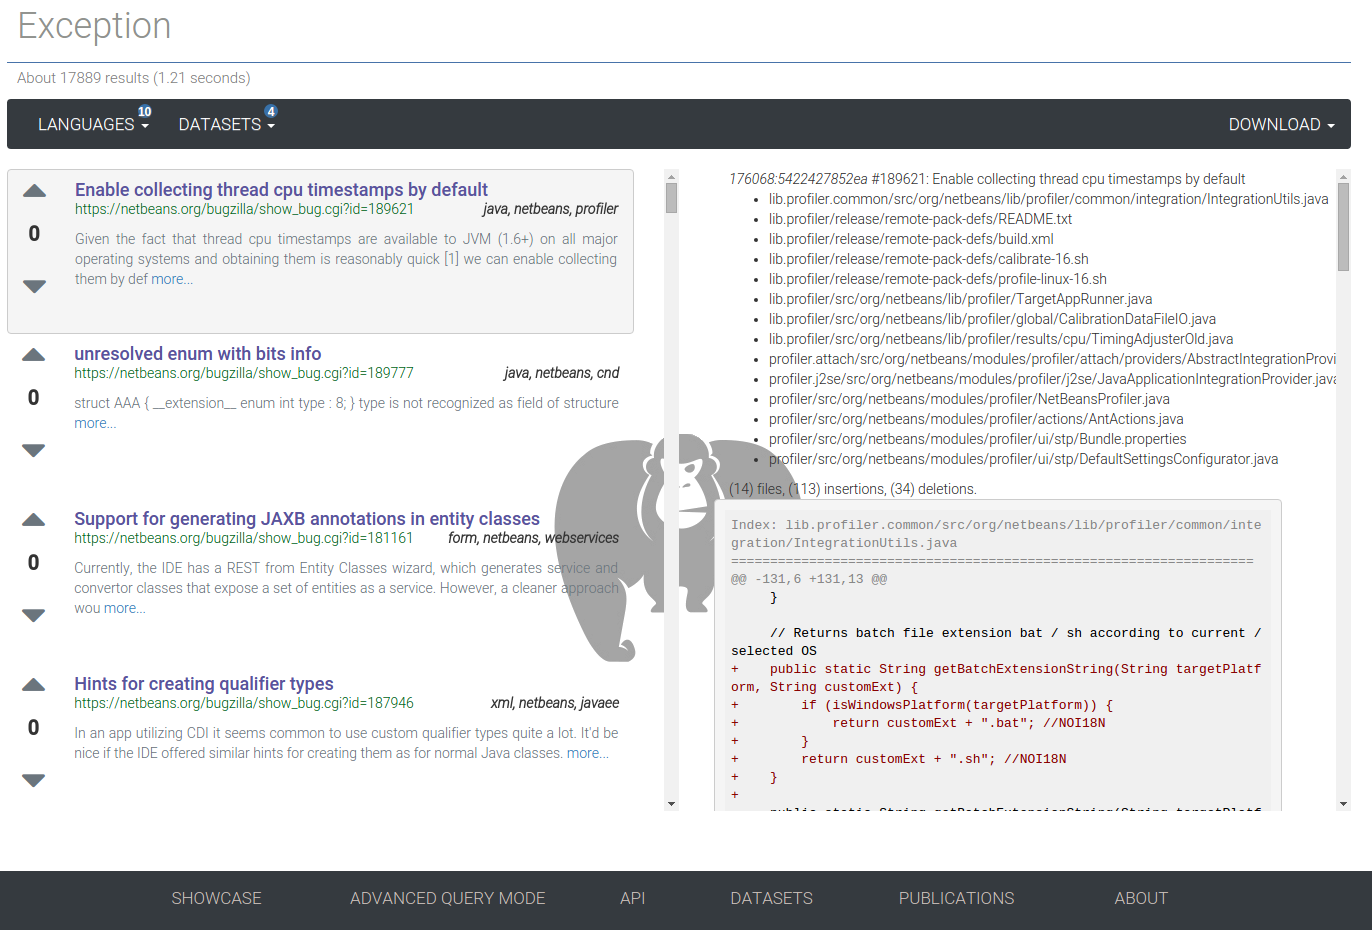
\includegraphics[scale=0.3]{media/bumper-live.png}
    \caption{Screenshot of https://bumper-app.com with ``Exception'' as research.
    \label{fig:bumper-live}}
\end{figure}


Moreover, BUMPER supports AND, OR, NOR operators and provide results in order of seconds.

As we said before, BUMPER is based on Apache Solr which have an incredibly rich API that is available online\footnote{ http://lucene.apache.org/solr/resources.html}.

{\tt BUMPER} serves as data repositories for the upcoming approaches presented in the chapters.

%!TEX root = ../research_proposal.tex

\section{JCHARMING - Java CrasH Automatic Reproduction by directed Model checkING\label{sec:JCHARMING}}

Field failures are challenging to reproduce because
the data provided by the end users is often scarce. A survey
conducted with developers of major open source software
systems such as Apache, Mozilla and Eclipse revealed that
one of the most valuable piece of information that can help
locate and fix the cause of a crash is the one that can help
reproduce it \cite{Bettenburg2008}. It is therefore important to invest in
techniques and tools for automatic bug reproduction to ease
the maintenance process and accelerate the rate of bug fixes
and patches.

In this section, we present an approach, called {\tt JCHARMING}
(Java CrasH Automatic Reproduction by directed Model
checkING) that uses a combination of crash traces and model
checking to automatically reproduce bugs that caused field
failures. Unlike existing techniques, such as on-field record and in-house replay \cite{Narayanasamy2005,Artzi2008,Jaygarl} or crash explanation \cite{Manevich2004,chandra2009snugglebug} JCHARMING does not
require instrumentation of the code. It does not need access to
the content of the heap either. Instead, JCHARMING uses a
list of functions output when an uncaught exception in Java
occurs (i.e., the crash trace) to guide a model checking engine
to uncover the statements that caused the crash. While we do not filter any personal information that may appear in the crash trace, JCHARMING  raises less privacy concerns than a tool recording every call or dump the content of the memory.

To assess the effiency of {\tt JCHARMING} we try to reproduce issues contained in {\tt BUMPER}.

\subsection{Preliminaries}

Model checking (also known as property checking) will, given a system (that could be software \cite{Visser2003} or hardware based \cite{kropf1999introduction}), check if the system meets a specification Spec by testing exhaustively all the states of the system under test (SUT), which can be represented by a Kripke \cite{Kripke1963} structure:

\begin{equation}
SUT = <S,T,P>
\end{equation}

where S is the set of states, $T \subseteq S * S$ represents the transitions between the states and P is the set of properties that each state satisfies. The SUT is said to satisfy a set of properties p when there exists a sequence of states transition x leading towards these properties. This can be written as:

\begin{equation}
(SUT, x)  \models p
\end{equation}

However, this only ensures that $\exists x$ such that $p$ is reached at some point in the execution of the program and not that $p$ holds nor that $\forall x$, $p$ is satisfiable. In JCHARMING, SUTs are bound to a simple specification: they must not crash under a fair environment. In the framework of this study, we consider a fair environment as any environment where the transitions between the states represent the functionalities offered by the program. For example, in a fair environment, the program heap or other memory spaces cannot be modified. Without this fairness constraint, all programs could be tagged as buggy since we could, for example, destroy objects in memory while the program continues its execution. As we are interested in verifying the absence of unhandled exceptions in the SUT, we aim to verify that for all possible combinations of states and transitions there is no path leading towards a crash. That is:

\begin{equation}
\forall x.(SUT, x) \models \neg c
\end{equation}

If such a path exists (i.e., $\exists x$  such that $(SUT, x)  \models c$) then the model checker engine will output the path $x$ (known as the counter-example) which can then be executed. The resulting Java exception crash trace is compared with the original crash trace to assess if the bug is reproduced. While  being  accurate and exhaustive in finding counter-examples, model checking suffers from the state explosion problem, which hinders its applicability to large software systems.


To show the contrast between testing and model checking, we use the hypothetical example of Figures \ref{fig:testing-toy}, \ref{fig:checking-toy} and \ref{fig:dchecking-toy} to sketch the possible results of each approach. These figures depicts a toy program where from the entry point, unknown calls are made (dotted points) and, at some points, two methods are called. These methods, called \texttt{Foo.Bar} and \texttt{Bar.Foo}, implement a for \texttt{loop} from 0 to \texttt{loopCount}. The only difference between these two methods is that the \texttt{Bar.Foo} method throws an exception if i becomes larger than two. Hereafter, we denote this property as $c_{i > 2}$.  


\begin{figure}[h!]
  \centering
    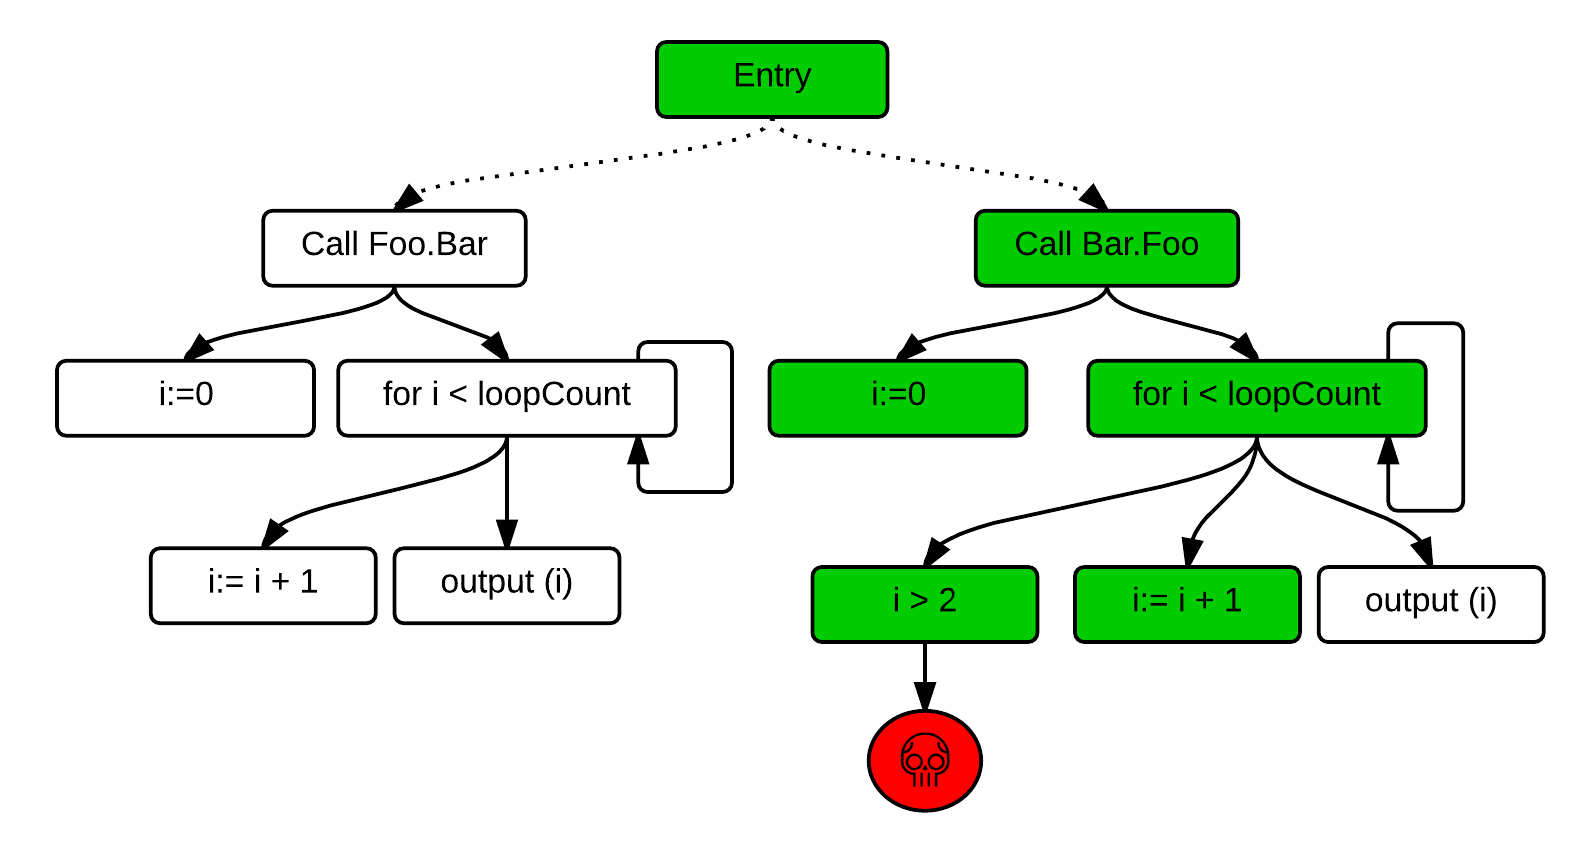
\includegraphics{media/dmc.png}
    \caption{A toy program under testing
    \label{fig:testing-toy}}
\end{figure}

\begin{figure}[h!]
  \centering
    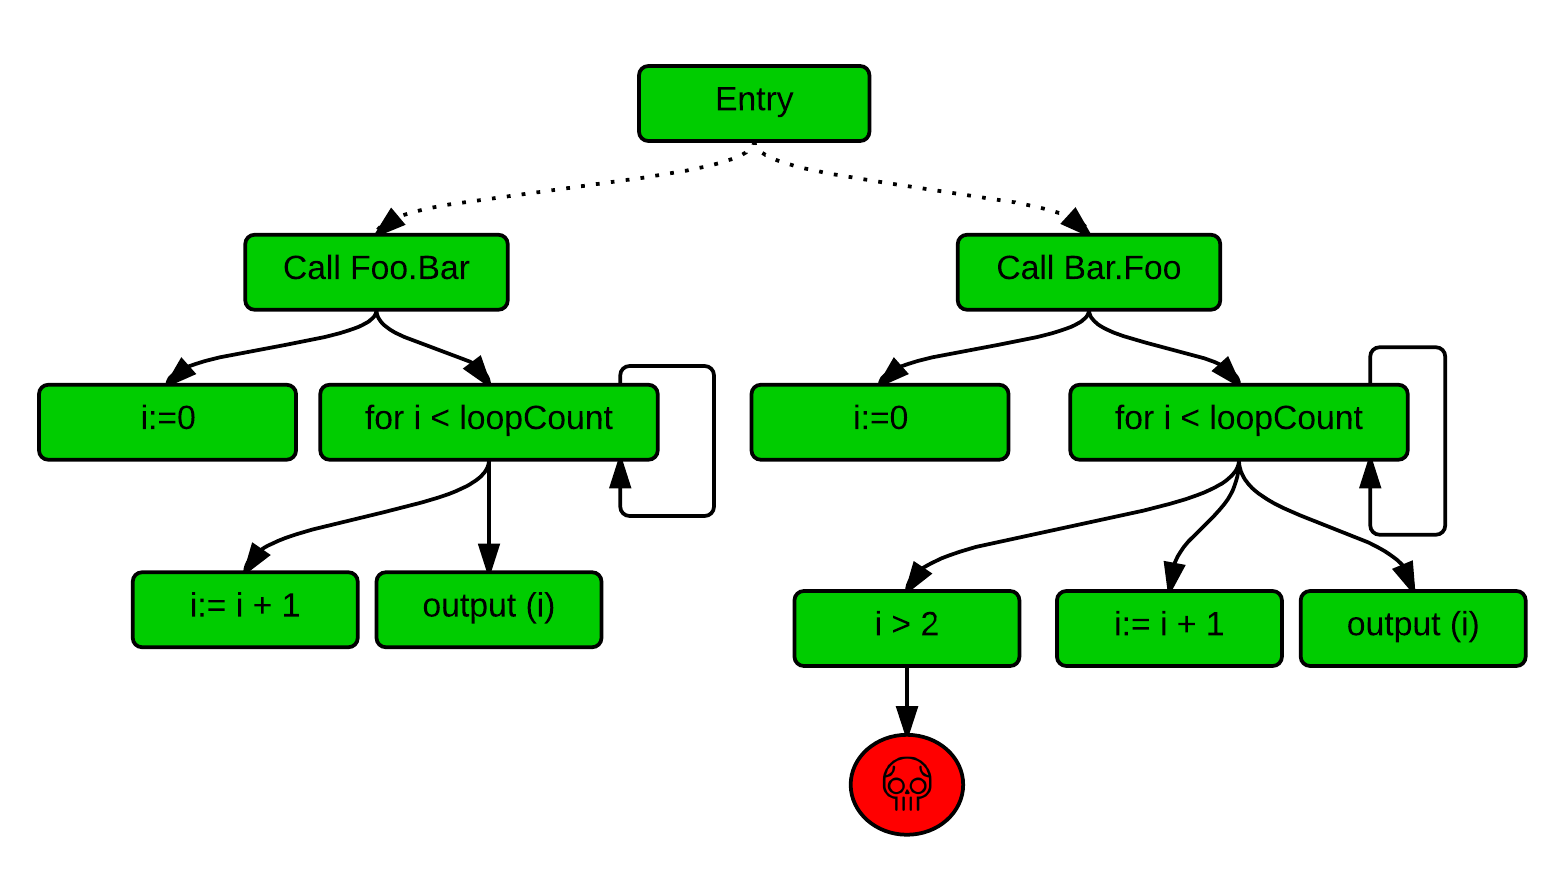
\includegraphics{media/mc.png}
    \caption{A toy program under model checking
    \label{fig:checking-toy}}
\end{figure}

\begin{figure}[h!]
  \centering
    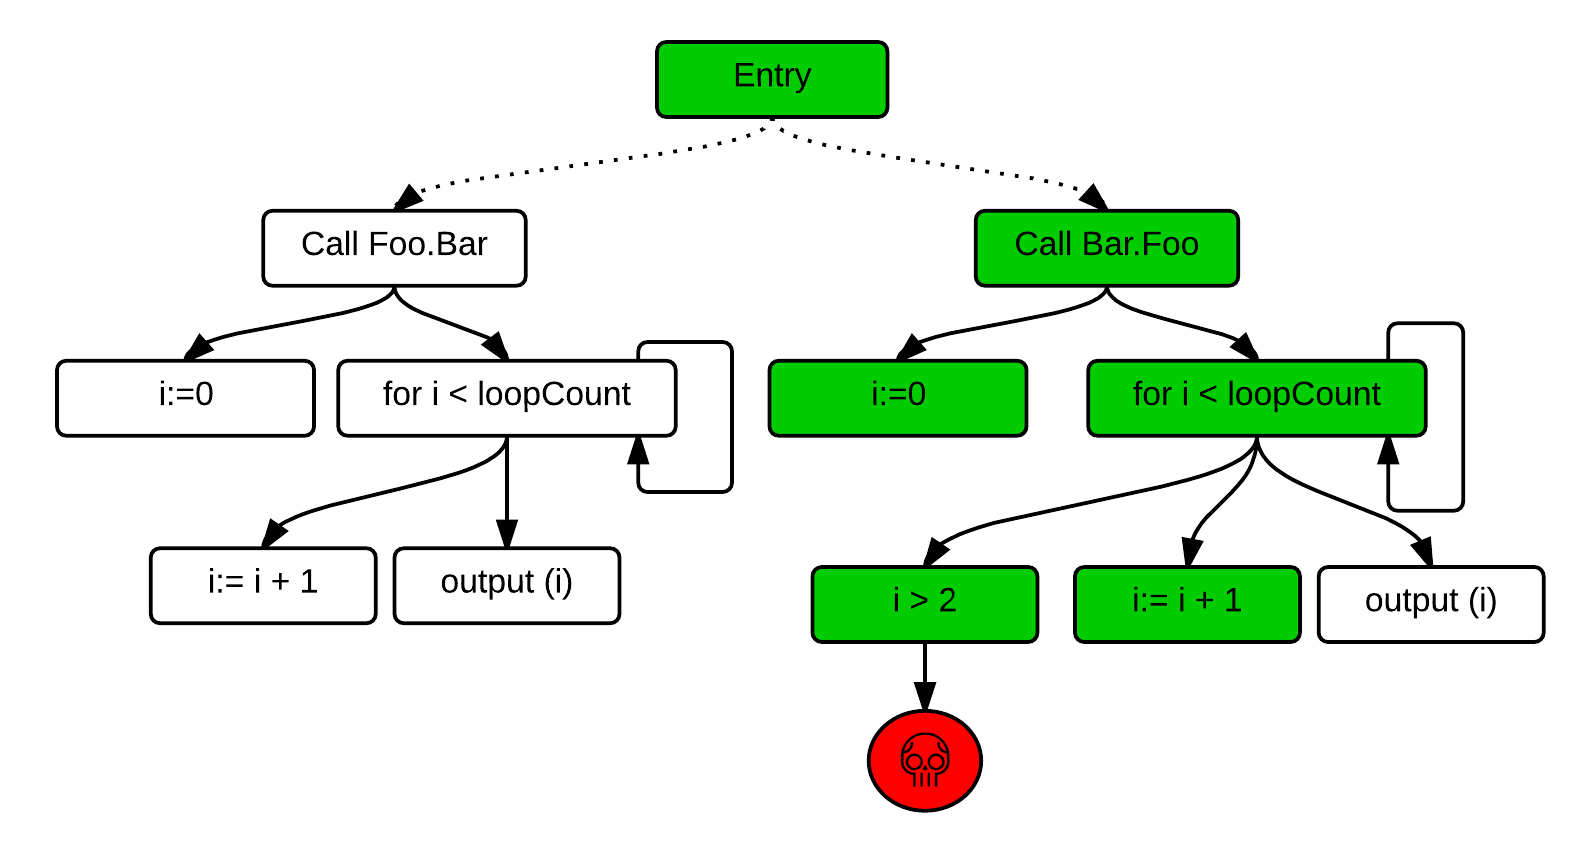
\includegraphics{media/dmc.png}
    \caption{A toy program under directed model checking
    \label{fig:dchecking-toy}}
\end{figure}

Figure \ref{fig:testing-toy} shows the program statements that could be covered using testing approaches. Testing software is a demanding task where a set of techniques is used to test the SUT according to some input.

Software testing depends on how well the tester understands the SUT in order to write relevant test cases that are likely to find errors in the program. Program testing is usually insufficient because it is not exhaustive. In our case, using testing would mean that the tester knows what to look for in order to detect the causes of the failure. We do not assume this knowledge in JCHARMING. 

Model checking, on the other hand, explores each and every state of the program (Figure \ref{fig:checking-toy}), which makes it complete, but impractical for real-world and large systems. To overcome the state explosion problem of model checking, directed (or guided) model checking has been introduced \cite{Rungta2009}. Directed model checking use insights—generally heuristics—about the SUT in order to reduce the number of states that need to be examined. Figure \ref{fig:dchecking-toy} explores only the states that may lead to a specific location, in our case, the location of the fault. The challenge, however, is to design techniques that can guide the model checking engine. As we will describe in the next section, we use crash traces and program slicing to overcome this challenge.

\subsection{The JCHARMING Approach}

Figure \ref{fig:jcarming-approach} shows an overview of JCHARMING. The first step
consists of collecting crash traces, which contain raw lines
displayed to the standard output when an uncaught exception
in Java occurs. In the second step, the crash traces are
preprocessed by removing noise (mainly calls to Java standard
library methods). The next step is to apply backward slicing
using static analysis to expand the information contained in
the crash trace while reducing the search space. The resulting
slice along with the crash trace are given as input to the model
checking engine. The model checker executes statements
along the paths from the main function to the first line of the
crash trace (i.e., the last method executed at crash time, also
called the crash location point). Once the model checker finds
inconsistencies in the program leading to a crash, we take the
crash stack generated by the model checker and compare it to
the original crash trace (after preprocessing). The last step is
to build a JUnit test, to be used by software engineers to
reproduce the bug in a deterministic way.

\begin{figure}[h!]
  \centering
    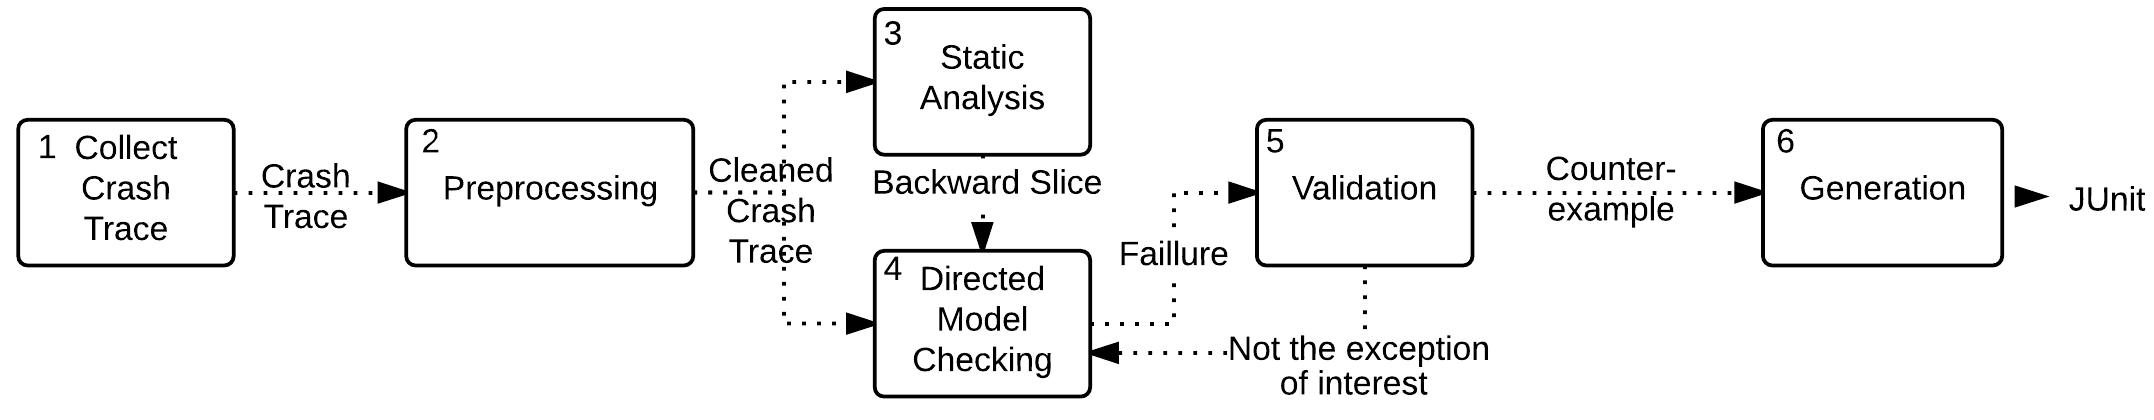
\includegraphics[scale=0.8]{media/jcharming-approach.png}
    \caption{Overview of JCHARMING.
    \label{fig:jcarming-approach}}
\end{figure}

\subsubsection{Collecting Crash Traces}

The first step of JCHARMING is to collect the crash trace
caused by an uncaught exception. Crash traces are usually included in crash reports and can therefore be automatically
retrieved using a simple regular expression.
Figure \ref{fig:jcarming-traces} shows an example of a crash trace that contains the
exception thrown when executing the program depicted in
Figures \ref{fig:testing-toy} to \ref{fig:dchecking-toy}. The crash trace contains a call to the Bar.foo()
method—the crash location point—and calls to Java standard
library functions (in this case, GUI methods because the
program was launched using a GUI).

\begin{figure}[h!]
  \noindent\fbox{%
      \parbox{\textwidth}{%
  1.javax.activity.InvalidActivityException:loopTimes \\
  should be < 3 \\
  2. at Foo.bar(Foo.java:10) \\
  3. at GUI.buttonActionPerformed(GUI.java:88) \\
  4. at GUI.access$0(GUI.java:85) \\
  5. at GUI$1.actionPerformed(GUI.java:57) \\
  6. caused by java.lang.IndexOutOfBoundsException : 3 \\
  7. at scam.Foo.buggy(Foo.java:17) \\
  8. and 4 more ...
      }%
  }
    \caption{Java InvalidActivityException is thrown in the Bar.Goo loop if the control variable is greater than 2.
    \label{fig:jcarming-traces}}
\end{figure}

As shown in Figure \ref{fig:jcarming-traces}, we can see that the first line (referred to
as frame {\it $f_0$} , subsequently the next line is called frame {\it $f_1$} , etc.)
does not represent the real crash point but it is only the last
exception of a chain of exceptions. Indeed, the {\tt InvalidActivity}
has been triggered by an {\tt IndexOutOfBoundsException} in
{\tt scam.Foo.buggy} . This kind of crash traces reflects several
nested try/catch blocks.

In addition, it is common in Java to have incomplete crash
traces. According to the Java documentation \cite{Oracle2011}, line 8 of
Figure \ref{fig:jcarming-traces} should be interpreted as follows: {\it ``This line indicates
that the remainder of the stack trace for this exception
matches the indicated number of frames from the bottom of the
stack trace of the exception that was caused by this exception
(the ``enclosing exception''). This shorthand can greatly
reduce the length of the output in the common case where a
wrapped exception is thrown from the same method as the
``causative exception'' is caught.}''

We are likely to find shortened traces in bug repositories as
they are what the user sees without any possibility to expand
their content.

\subsubsection{Preprocessing}

In the preprocessing step, we first reconstruct and reorganize
the crash trace in order to address the problem of nested
exceptions. Then, with the aim to obtain an optimal guidancefor our directed model checking engine, we remove frames
that are out of our control. Frames out of our controls refer
usually, but are not limited to, Java library methods and third
party libraries. In Figure \ref{fig:jcarming-traces}, we can see that Java GUI and
event management components appear in the crash trace. We
assume that these methods are not the cause of the crash;
otherwise it means that there is something wrong with the on-
field JDK. If this is the case, we will not be able to reproduce
the crash. Note that removing these unneeded frames will also
reduce the search space of the model checker.

\subsubsection{Building the Backward Static Slice}

For large systems, a crash trace does not necessary contain all
the methods that have been executed starting from the entry
point of the program (i.e., the main function) to the crash
location point. We need to complete the content of the crash
trace by identifying all the statements that have been executed
starting from the main function until the last line of the
preprocessed crash trace. In Figure \ref{fig:jcarming-traces}, this will be the function
call {\tt Bar.foo()}, which happens to be also the crash location
point. To achieve this, we turn to static analysis by extracting
a backward slice from the main function of the program to the
{\tt Bar.foo()} method.

A backward slice contains all possible branches that may lead
to a point {\it n} from a point {\it m} as well as the definition of the
variables that control these branches \cite{de2001program}. In other words, the
slice of a program point {\it n} is the program subset that may
influence the reachability of point {\it n} starting from point {\it m}.
The backward slice containing the branches and the definition
of the variables leading to {\it n} from {\it m} is noted as {\it $bslice_{[m \leftarrow n]}$}.

We perform a static backward slice between each frame to
compensate for possible missing information in the crash
trace. More formally, the final static backward slice is
represented as follows:

\begin{equation}
\centering
\begin{split}
bslice_{[entry \leftarrow f_0]} = bslice_{[f_1 \leftarrow f_0]} \cup bslice_{[f_2 \leftarrow f_1]} \cup ... \cup bslice_{[f_n \leftarrow f_{n−1}]} \cup bslice_{[entry \leftarrow f_n]}
\end{split}
\end{equation}

Note that the union of the slices computed between each pair
of frames must be a subset of the final slice between $f_0$ and the
entry point of the program. More formally:

\begin{equation}
\centering
\begin{split}
\bigcup_{i=0}^{entry} bslice_{[f_{i+1} \leftarrow f_i]} \subseteq bslice_{[entry \leftarrow f_0]}
\end{split}
\end{equation}

Indeed, in Figure \ref{fig:jcharming-slice}, the set of states allowing to reach $f_0$ from
$f_2$ is greater than the set of states to reach $f_1$ from $f_2$ plus set
of states to reach $f_0$ from $f_1$ . In this hypothetical example and
assuming that $z_2$ is a prerequisite to $f_2$ then
$bslice_{[entry \leftarrow f_0]} = \{f_0 , f_1 , f_2 , z_0 , z_1 , z_2 , z_3 \}$
while $\cup_{i=0}^n bslice_{[f_{i+1} \leftarrow f_i]}$.

\begin{figure}[h!]
  \centering
    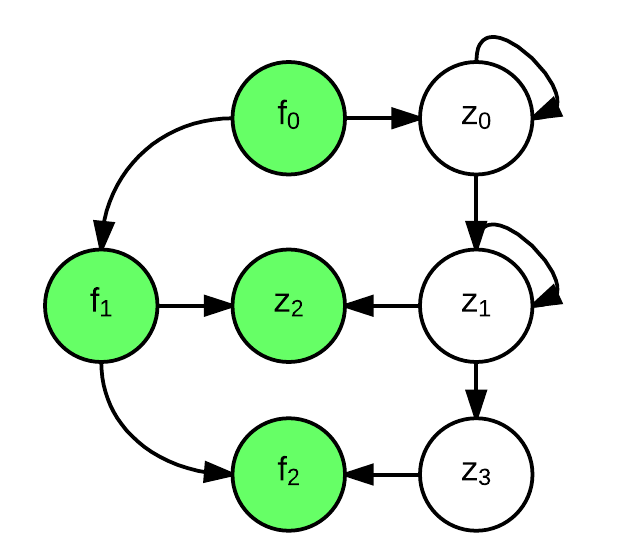
\includegraphics{media/jcharming-slices.png}
    \caption{Hypothetical example representing $bslice_{[entry \leftarrow f_0]}$ Vs. $\cup_{i=0}^n bslice_{[f_{i+1} \leftarrow f_i]} = \{f_0 , f_1 , f_2 , z_2 \}$
    \label{fig:jcharming-slice}}
\end{figure}

In the worst case scenerio where there exists one and only one
transition between each frame, which is very unlikely for real
and complex systems, then $bslice_{[entry \leftarrow f_0]}$ and
 $\cup_{i=0}^n bslice_{[f_{i+1} \leftarrow f_i]}$ yield the same set of states with a
comparable computational cost since the number of branches
to explore will be the same in both cases.

Algorithm \ref{alg:jcharming-slice} is a high level
representation of how we compute the backward slice between
each frame. The algorithm takes as input the pre-processed
call trace, the byte code of the SUT, and the entry point. From
line 1 to line 5, we initialize the different variables used by the
algorithm. The main loop of the algorithm begins at line 6 and
ends at line 15. In this loop, we compute the static slice
between the current frame and the next one. If the computed
static slice is not empty then we update the final backward
slice with the newly computed slice.


\begin{algorithm}[H]
 \KwData{Crash Stack, BCode, Entry Point}
 \KwResult{BSolve}
 $Frames~frames~\leftarrow~extract~frames~from~crash~stack$\;
 Int n $\leftarrow$ size of frame\;
 Int offset $\leftarrow$ 1\;
 Bslice bSlice $\leftarrow$ $\emptyset$\;
\For{i $\leftarrow$ 0 to i $<$ n \&\& offset $<$ n - 1}{
  BSlice currentBSlice $\leftarrow$ backward slice from frames[i] to i + offset\;
  \eIf{currentBSlice $\not=$ $\emptyset$}{
   bSlice $\leftarrow$ bSlice $\cup$ currentBSlice\;
   offset $\leftarrow$ 1\;
  }{
   offset $\leftarrow$ offset +1\;
  }
}
\caption{High level algorithm computing the union of the slices\label{alg:jcharming-slice}}
\end{algorithm}

Using backward slicing, the search space of the model checker
that processes the example of Figures \ref{fig:testing-toy} to \ref{fig:dchecking-toy} is given by the
following expression:

\begin{equation}
  \exists x.
  \begin{pmatrix}
    \bigcup_{i=0}^{entry} bslice_{[f_{i+1} \leftarrow f_i]}  \subset SUT \\
    x.\bigcup_{i=0}^{entry} bslice_{[f_{i+1} \leftarrow f_i]}  \subset x.SUT
  \end{pmatrix}
  \models c_{i>2}
\end{equation}

That is, there exists a sequence of states transitions $x$ that
satisfies $c_{i>2}$ where both the transitions and the states are
entry
elements of $\bigcup_{i=0}^{entry} bslice_{[f_{i+1} \leftarrow f_i]}$ . Obviously, $c_{i>2}$ also
needs to be included for the final static slice to be usable by
the model checking engine. Consequently, the only frame that
need to be untouched for the backward static slice to be
meaningful is $f_0$.

\subsubsection{Directed Model Checking}

The model checking engine we use in this paper is called JPF
(Java PathFinder) \cite{Visser2004}, which is an extensible JVM for Java
bytecode verification. This tool was first created as a front-end
for the SPIN model checker \cite{holzmann1997model} in 1999 before being open-
sourced in 2005. JPF is organized around five simple
operations: (i) {\it generate states}, (ii) {\it forward}, (iii) {\it backtrack},
(iv) {\it restore state} and (v) {\it check}. In the forward operation, the
model checking engine generates the next state $s_{t+1}$ . If
$s_{t+1}$ has successors then it is saved in a backtrack table to be
restored later. The backtrack operation consists of restoring
the last state in the backtrack table. The restore operation
allows restoring any state and can be used to restore the entire
program as it was the last time we choose between two
branches. After each, forward, backtrack and restore state
operation the check properties operation is triggered.

In order to direct JPF, we have to modify the {\it generate states}
and the {\it forward} steps. The {\it generate states} is populated with
entry
the states in $\bigcup_{i=0}^{entry} bslice_{[f_{i+1} \leftarrow f_i]}  \subset SUT$ and we adjust the
{\it forward step} to explore a state if the target state $s_i+1$ and the
transition $x$ to pass from the current state $s_i$ to $s_{i+1}$ are in
$\bigcup_{i=0}^{entry} bslice_{[f_{i+1} \leftarrow f_i]}  \subset SUT$ and $x.\bigcup_{i=0}^{entry} bslice_{[f_{i+1} \leftarrow f_i]}  \subset x.SUT$.

\subsubsection{Validation}

To validate the result of directed model checking, we modify
the {\it check properties} step that checks if the current sequence
of states transitions $x$ satisfies a set a property. If the current
states transitions $x$ can throw an exception, we execute $x$ and
compare the exception thrown to the original crash trace (after
preprocessing). If the two exceptions match, we conclude that
the conditions needed to trigger the failure have been met and
the bug is reproduced.

However, as argued by Kim et al. in \cite{Kim2013b}, the same failure can
be reached from different paths of the program. Although the
states executed to reach the defect are not exactly the same,
they might be useful to enhance the understanding of the bug
by software developers, and speed up the deployment of a fix.
Therefore, in this paper, we consider a defect to be partially
reproduced if the crash trace generated from the model
checker matches the original crash trace by a factor of $t$, where
$t$ is a threshold specified by the user. $t$ is the percentage of
identical frames between both crash traces.

\subsubsection{Generating Test Cases for Bug Reproduction}

To help software developers reproduce the crash in a lab
environment we automatically produce the JUnit test cases
necessary to run the SUT to cause the exercise of the bug.

To build a test suite that reproduces a defect, we need to create
a set of objects used as arguments for the methods that will
enable us to travel from the entry point of the program to the
defect location. JPF has the ability to keep track of what
happens during model checking in the form of traces
containing the visited states and the value of the variables. We
leverage this capability to create the required objects and call
the methods leading to the failure location. Although we can
track back the internal state of objects at a specific time using
JPF, it can be too computationally taxing to recreate only the
objects needed to generate the bug. To overcome this, we use
serialization techniques \cite{Opyrchal1999}. We take advantage of features
offered by the XStream \cite{Xstream2011} library which enables the
serialization and deserialization of any Java object — even
objects that do not implement the Java Serializable interface.
We use the serialization when the model checker engine
performs too many operations modifying the property of a
given object. In such case, we serialize the last state of the
object.

\subsection{Case studies}

In this section, we show the effectiveness of JCHARMING to
reproduce bugs in seven open source systems\footnote{The bug reports used in this study and the result of the model checker are
made available for download from research.mathieu-
nayrolles.com/jcharming/} . The aim of the
case study is to answer the following question: {\it Can we use
crash traces and directed model checking to reproduce on-
field bugs in a reasonable amount of time?}

\subsubsection{Targeted Systems}

Table \ref{tab:jacharming-systems} shows the systems and their characteristics in terms of
Kilo Line of Code (KLoC) and Number of Classes (NoC).

\begin{table}[h!]
\centering
\begin{tabular}{c|c|c|c}
SUT        & KLOC & NoC  & Bug \#ID                                        \\ \hline \hline
Ant        & 265  & 1233 & 38622, 41422                                    \\
ArgoUML    & 58   & 1922 & 2603, 2558, 311, 1786                           \\
dnsjava    & 33   & 182  & 38                                              \\
jfreechart & 310  & 990  & 434, 664, 916                                   \\
Log4j      & 70   & 363  & 11570, 40212, 41186, 45335, 46271, 47912, 47957 \\
MCT        & 203  & 1267 & 440ed48                                         \\
pdfbox     & 201  & 957  & 1412, 1359 \\ \hline \hline
\end{tabular}
\caption{List of taget systems in terms of Kilo line of code (KLoC), number of classes (NoC) and Bug \# ID}
\label{tab:jacharming-systems}
\end{table}

Apache Ant \cite{ApacheSoftwareFoundation} is a popular command-line tool to build
make files. While it is mainly known for Java applications,
Apache Ant also allows building C and C++ applications. We
choose to analyze Apache Ant because it has been used by
other researchers in similar studies.

ArgoUML \cite{CollabNet} is one of the major players in the open source
UML modeling tools. It has many years of bug management
and, similar to Apache Ant, it has been extensively used as a
test subject in many studies.

Dnsjava \cite{Wellington2013} is a tool for the implementation of the DNS
mechanisms in Java. This tool can be used for queries, zone
transfers, and dynamic updates. It is not as large as the other
two, but it still makes an interesting case subject because it has
been well maintained for the past decade. Also, this tool is
used in many other popular tools such as Aspirin, Muffin and
Scarab.

JfreeChart \cite{ObjectRefineryLimited2005} is a well-known library that enables the
creation of professional charts. Similar to dnsjava, it has been
maintained over a very long period of time —JfreeChart was
created in 2005— and it is a relatively large application.

Apache Log4j \cite{TheApacheSoftwareFoundation1999} is a logging library for Java. This is not a
very large library, but it is extensively used by thousands of
programs. As other Apache projects, this tool is well
maintained by a strong open source community and allows
developers to submit bugs. The bugs which are in the bug
report system of Log4j are, generally speaking, well
documented and almost every bug contains a related crash
trace and, therefore, it is a tool of interest to us.

MCT \cite{NASA2009} stands for Mission Control technologies and was
developed by the NASA Ames Research Center (the creators
of JPF) for use in spaceflight mission operation. This tool
benefits from two years of history and targets a very critical
domain, Spacial Mission Control. Therefore, this tool has to
be particularly and carefully tested and, consequently, the
remaining bugs should be hard to discover and reproduce.

PDFBox \cite{ApacheSoftwareFoundation2014} is another tool supported by the Apache
Software Foundation since 2009 and was created in 2008.
PDFBox allows the creation of new PDF documents and the
manipulation of existing documents.

\subsubsection{Bug Selection and Crash Traces}

In this study, we have selected the reproduced bugs randomly
in order to avoid the introduction of any bias. We selected a
random number of bugs ranging from 1 to 10 for each SUT
containing the word ``exception'' and where the description of
the bug contains a match a regular expression designed to find the pattern of a
Java exception.

\subsection{Results}

Table \ref{tab:jcharming-results} shows the results of JCHARMING in terms of Bug
\#ID, reproduction status, and execution time (in minutes) of
directed model checking (DMC) and Model Checking (MC).
The experiments have been conducted on a Linux machine (8
GB of RAM and using Java 1.7.0\_51).

\begin{itemize}
  \item The result is noted as ``Yes'' if the bug has been fully
reproduced, meaning that the crash trace generated by the
model checker is identical to the crash trace collected
during the failure of the system.
\item The result is ``Partial'' if the similarity between the crash
trace generated by the model checker and the original
crash trace is above t=80\%. Given an 80\% similarity
threshold, we consider partial reproduction as successful.
A different threshold could be used.
\item Finally, the result of the approach is reported as ``No'' if
either the similarity is below t < 80\% or the model
checker failed to crash the system given the input we
provided.
\end{itemize}

\begin{table}[h!]
\centering
\begin{tabular}{c|c|c|c|c}
SUT                         & Bug \#ID & Reprod. & Time DMC & Time MC \\ \hline \hline
\multirow{2}{*}{Ant}        & 38622    & Yes     & 25.4     & -       \\
                            & 41422    & No      & -        & -       \\ \hline
\multirow{4}{*}{ArgoUML}    & 2558     & Partial & 10.6     & -       \\
                            & 2603     & Partial & 9.4      & -       \\
                            & 311      & Yes     & 11.3     & -       \\
                            & 1786     & Partial & 9.9      & -       \\  \hline
DnsJava                     & 38       & Yes     & 4        & 23      \\ \hline
\multirow{3}{*}{jFreeChart} & 434      & Yes     & 27.3     & -       \\
                            & 664      & Partial & 31.2     & -       \\
                            & 916      & Yes     & 26.4     & -       \\ \hline
\multirow{7}{*}{Log4j}      & 11570    & Yes     & 12.1     & -       \\
                            & 40212    & Yes     & 15.8     & -       \\
                            & 41186    & Partial & 16.7     & -       \\
                            & 45335    & No      & -        & -       \\
                            & 46271    & Yes     & 13.9    & -       \\
                            & 47912    & Yes     & 12.3     & -       \\
                            & 47957    & No      & -        & -       \\
MCT                         & 440ed48  & Yes     & 18.6     & -       \\ \hline
\multirow{2}{*}{PDFBox}     & 1412     & Partial & 19.7     & -       \\
                            & 1359     & No      & -        & - \\ \hline \hline
\end{tabular}

\caption{Effectiveness of JCHARMING using directed model checking (DMC) and model checking (MC) in minutes}
\label{tab:jcharming-results}
\end{table}

As we can see in Table \ref{tab:jcharming-results}, we were able to reproduce 17 bugs
out of 20 bugs either completely or partially (85% success
ratio). The average time to reproduce a bug is 16 minutes.
This result demonstrates the effectiveness of our approach,
more particularly, the use of backward slicing to create a
manageable search space that guides adequately the model
checking engine. We also believe that our approach is usable
in practice since it is also time efficient. Among the 20 different bugs we have tested, we will describe
one bug (chosen randomly) for each category (successfully
reproduced, partially reproduced, and not reproduced) for
further analysis.

\subsubsection{Successfully reproduced}

The first bug we describe in this discussion is the bug \#311
belonging to ArgoUML. This bug was submitted in an earlier
version of ArgoUML. This bug is very simple to manually
reproduce thanks to the extensive description provided by the
reporter, which reads: {\it ``I open my first project (Untitled Model by default). I choose
to draw a Class Diagram. I add a class to the diagram. The
class name appears in the left browser panel. I can select the
class by clicking on its name. I add an instance variable to the
class. The attribute name appears in the left browser panel. I
can't select the attribute by clicking on its name. Exception
occurred during event dispatching:''}

The reporter also attached the following crash trace that we
used as input for JCHARMING:

\noindent\fbox{%
    \parbox{\textwidth}{%
1. java.lang.NullPointerException:\\
2. at\\
3. uci.uml.ui.props.PropPanelAttribute
.setTargetInternal (PropPanelAttribute.java)\\
4. at uci.uml.ui.props.PropPanel.
setTarget(PropPanel.java)\\
5. at uci.uml.ui.TabProps.setTarget(TabProps.java)\\
6. at uci.uml.ui.DetailsPane.setTarget
(DetailsPane.java)\\
7. at uci.uml.ui.ProjectBrowser.select
(ProjectBrowser.java)\\
8. at uci.uml.ui.NavigatorPane.mySingleClick
(NavigatorPane.java)\\
9. at uci.uml.ui.NavigatorPane\$Navigator
MouseListener.mouse Clicked(NavigatorPane.java)\\
10.at
java.awt.AWTEventMulticaster.mouseClicked
(AWTEventMulticaster.java:211)\\
11.
at
java.awt.AWTEventMulticaster.mouseClicked
(AWTEvent
Multicast er.java:210)\\
12.at
java.awt.Component.processMouseEvent
(Component.java:3168)\\
...\\
19. java.awt.LightweightDispatcher
.retargetMouseEvent (Container.java:2068)\\
22.
at java.awt.Container
.dispatchEventImp l(Container.java:1046)\\
23.
at java.awt.Window
.dispatchEventImpl (Window.java:749)\\
24.
at java.awt.Component
.dispatchEvent (Component.java:2312)\\
25.
at java.awt.EventQueue
.dispatchEvent (EventQueue.java:301)\\
28.
at java.awt.EventDispatchThread.pumpEvents\\
(EventDispatch Thread.java:90)
29.
at java.awt.EventDispatchThread.run(EventDispatch
Thread.java:82)
    }%
}

The cause of this bug is that the reference to the attribute of
the class was lost after being displayed on the left panel of
ArgoUML and therefore, selecting it through a mouse click
throws a null pointer exception. In the subsequent version,
ArgoUML developers added a TargetManager to keep the
reference of such object in the program. Using the crash trace, JCHARMING's preprocessing step
removed the lines between lines 11 and 29 because they
belong to the Java standard library and we do not want neither
the static slice nor the model checking engine to verify the
Java standard library but only the SUT. Then, the third step
performs the static analysis following the process described in
Section IV.C. The fourth step performs the model checking on
the static slice to produce the same crash trace. More
specifically, the model checker identifies that the method
{\tt setTargetInternal(Object o)} could receive a null object that
will result in a {\tt Null} pointer exception.

\subsubsection{Partially reproduced}

As an example of a partially reproduced bug, we explore the
bug \#664 of the Jfreechart program. The description provided
by the reporter is: ``{\it In ChartPanel.mouseMoved there's a line
of code which creates a new ChartMouseEvent using as first
parameter the object returned by getChart(). For getChart() is
legal to return null if the chart is null, but ChartMouseEvent's
constructor calls the parent constructor which throws an
IllegalArgumentException if the object passed in is null.}''

The reporter provided the crash trace containing 42 lines and
the replaced an unknown number of lines by the following
statement ``<deleted entry>''. While JCHARMING successfully reproduced a crash yielding almost the same trace
as the original trace, the ``<deleted entry>'' statement -- which
was surrounded by calls to the standard java library -- was not
suppressed and stayed in the crash trace. That is,
JCHARMING produced only the 6 (out of 7) first lines and
reached 83\% similarity, and thus a partial reproduction.

\noindent\fbox{%
    \parbox{\textwidth}{%

1. java.lang.IllegalArgumentException: null source\\
2. at java.util.EventObject.<init>(
EventObject.java:38)\\
3. at\\
4 org.jfree.chart.ChartMouseEvent.<init>
(ChartMouseEvent.java:83)\\
5. at org.jfree.chart.ChartPanel
.mouseMoved(ChartPanel.java:1692)\\
6. $<$deleted entry$>$

    }%
}

In all bugs that were partially reproduced, we found that the
differences between the crash trace generated from the model
checker and the original crash trace (after preprocessing)
consists of few lines only.

\subsubsection{Not Reproduced}

To conclude the discussion on the case study, we present a
case where JCHARMING was unable to reproduce the failure.
For the bug \#47957 belonging to Log4j and reported in late
2009 the reporter wrote: ``{\it Configure SyslogAppender with a Layout class that does not
exist; it throws a NullPointerException. Following is the
exception trace:}'' and attached the following crash trace:

\noindent\fbox{%
    \parbox{\textwidth}{%

1. 10052009 01:36:46 ERROR [Default: 1]
struts.CPExceptionHandler.execute
RID[(null;25KbxlK0voima4h00ZLBQFC;236Al8E60000045C3A
7D74272C4B4A61)] \\
2. Wrapping Exception in ModuleException\\
3. java.lang.NullPointerException\\
4. at org.apache.log4j.net.SyslogAppender
.append(SyslogAppender.java:250)\\
5. at org.apache.log4j.AppenderSkeleton
.doAppend(AppenderSkeleton.java:230)\\
6. at org.apache.log4j.helper.AppenderAttachableImpl
.appendLoopOnAppenders(AppenderAttachableImpl
.java:65)\\
7. at org.apache.log4j.Category.callAppenders
(Category.java:203)\\
8. at org.apache.log4j.Category
.forcedLog(Category.java:388)\\
9. at org.apache.log4j.Category.info
(Category.java:663)

    }%
}

The first three lines are not produced by the standard
execution of the SUT but by an ExceptionHandler belonging
to Struts \cite{ApacheSoftwareFoundation2000}. Struts is an open source MVC (Model View
Controller) framework for building Java Web Application.
JCHARMING examined the source code of Log4J for the
crash location {\tt struts.CPExceptionHandler.execute} and did not
find it since this method belongs to the source base of Struts
-- which uses log4j as a logging mechanism. As a result, the
backward slice was not produced, and we failed to perform the
next steps. It is noteworthy that the bug is marked as duplicate
of the bug \#46271 which contains a proper crash trace. We
believe that JCHARMING could have successfully
reproduced the crash, if it was applied to the original bug. \\

While JCHARMING is effective at reproducing on-field failures in lab environment, we want to reduce their number in the coming year. To do so, we built {\tt RESSEMBLE} and {\tt BIANCA} that we present in the next two sections.
%!TEX root = ../research_proposal.tex

\subsection{RESEMBLE - REcommendation System based on cochangE Mining at Block LEvel\label{sec:RESEMBLE}}

{\tt RESEMBLE} (REcommendation System based on cochangE Mining at Block LEvel) is a contextual recommendation system that will take the form of another pre-commit hook. {\tt RESEMBLE} will leverage the branches' history and the blocks extracted by {\tt PRECINCT} to identify, on the fly, sub-optimum or hazardous code and display and actual solution to the problem.


\subsubsection{Mining sequences of changes}

In the data mining field, ARM is a
well-established method for discovering co-occurrences between attributes
in the objects of a large data set \cite{Gregory1991,HEIKKI1997}. Plain
associations have the form $X \rightarrow Y$, where $X$ and $Y$,
called the \textit{antecedent} and the \textit{consequent}, respectively, are sets of descriptors
(purchases by a customer, network alarms, or any other general kind of events).
Even though plain association rules could serve some relevant information, we are interested here in
the sequences of changes that we believe will yield more precise result. Indeed, we think that similar modifications are often done in the same order by the same developer (e.g top to bottom or bottom to top).
We, therefore, adopt a variant called sequential association rules in which
both $X$ and $Y$ become sequences of descriptors.
Moreover, our sequences follow a temporal order with the antecedent preceding the consequent.
Rules of this type mined from changes reveal crucial
information about the likelihood of blocks of code to be modified together in a programming session
and, more importantly, in a specific order.
For instance, a strong rule \emph{$Block_A$ $,$ $Block_B$} implies \emph{$Block_C$} would mean that after modifying $Block_A$ and then $Block_B$, there are good chances that the developer needs to modify $Block_C$.
The conciseness of this example should not confuse the reader as in practical cases
the sequences appearing in a rule can be of an arbitrary length.
Furthermore, the strength of the rule is measured by the \textit{confidence} metric.
In probabilistic terms,
it measures the conditional probability of C appearing down the line.
Beside that, the significance of a rule, i.e. how many times it appears in the data, is provided by its \textit{support} measure.
To ensure only rules of potentially high interestingness are mined,
the mining task is tuned by minimal thresholds to
output only the sufficiently high scores for both metrics.

To extract the association rules from changes,
two choices were possible. On one hand, sequential pattern mining and rule mining algorithms
have been designed for structures that are slightly more general than the ones used here.
In fact, sequential patterns are defined on transactions that represent sequences of sets.
Efficient sequential pattern miners have been published, e.g. the PrefixSpan method \cite{Pei2004}.
On the other hand, sequence of changes do not compile to fully-blown sequential transactions as the underlying structures are mere sequences of individual elements. Such data has been known since at least the mid-90s but received less attention by the data mining community, arguably because it is less challenging to mine.
In the general data mining literature, mining from pure sequences, as opposed to sequences made of sets, has been addressed under the name of episode mining \cite{HEIKKI1997}.
Episodes are made of \textit{events} and in a sense, code changes are events. Arguably the largest body of knowledge on the subject belongs to the web usage mining field: The input data is again a system log, yet this time the log of requests sent to a web server \cite{Pei2000}.
It is noteworthy that sequential patterns are more general than the pure sequence ones, hence mining algorithms designed for the former might prove to be less efficient when applied to the latter (as additional steps might be required for listing all significant set).
Nevertheless, to jump-start our experimental study, we used a sequential pattern/rule miner that has the advantage to be freely available on the web\footnote{http://www.philippe-fournier-viger.com/spmf/}.
Although it has not been optimized for pure sequences its performances are more than satisfactory.

\subsubsection{Code Normalization\label{sec:resemble-normalization}}

Normalizing code is the action of making its structure consistent throughout the program according to a defined model. In our case, we only normalize the block of code that are in the current sequential association rules. To do so, we improve and combine several technologies such as source code transformation \cite{Cordy2006,Cordy2006a}, source code pretty-printing \cite{Roy2008}, flexible source code normalization \cite{Cordy2011}.

More specifically, the code first goes to a pretty printer. A pretty-printer is a component that will slightly transform the code in order to obtain consistent control structure.
Concretely, spaces will be added, accolade moved and tabulation added for an $if$, a $while$ and others structures to always appear the same way, regardless of the programming language.
Then, the code is normalized several times. Each normalization is different and targets specific feature of the code.
For example, we have one normalization that removes completely the variable names and replace the types by the highest known object in the object oriented hierarchy before {\tt Object} itself\footnote{For Java programs}. Another normalization only keeps the structures of the source code by normalizing both variables names and types.

\subsubsection{Comparing normalization\label{sec:resemble-comparing}}

Comparing different normalizations is the easiest step and can be done efficiently using using the longest common sequence (LCS) algorithm \cite{hirschberg1977algorithms}.
If the LCS is above an user-defined threshold, then a two different behaviors can be observed:

\begin{itemize}
	\item If the modified blocks' --- and potentially the ones that are likely to be modified after according to our sequential association rules --- normalizations match the normalizations of blocks of code that have been removed in past history. {\tt RESEMBLE} recommends the replacing code as a better solution.
  In other words, if blocks $A$, $B$ and $C$ have been replaced by blocks $A'$, $B'$ and $C'$ and blocks $D$, $E$ and $F$ normalizations match $A$, $B$ and $C$, then, {\tt RESEMBLE} recommends to transform $D$, $E$ and $F$ to look like $A'$, $B'$ and $C'$. This could lead to the introduction of software clones but we argue that (i) software clones are not always harmfull \cite{Juergens2009} and (ii) informing the developer that $A'$, $B'$ and $C'$ exist could lead him to re-use these blocks.
	\item If the modified blocks' --- and potentially of the ones that are likely to be modified after according to our sequential association rules --- normalizations match the normalization of blocks of code that are present in the history. {\tt RESEMBLE} computes the differences between the developer code and the history code in order to suggests what the developer have to do next.
\end{itemize}

\subsubsection{Planned experiments}

We did not started the experiments for {\tt RESEMBLE} yet. Nevertheless, we plan to conduct the following experiments:

\begin{itemize}
	\item Full history test with Normalization 1.
	\item Full history test with Normalization 2.
	\item An human study where:
	\begin{itemize}
		\item Developers use {\tt RESEMBLE} in order to determine whether or not developers take into account our recommendations to avoid inserting defects in the code.
		\item Developers use {\tt RESEMBLE} in order to determine whether or not developers take into account our recommendations to complete their modification according to what we found in the history.
		\item Rate the suggested solution in a scale from 1 to 10 in order to determine if the proposed change pattern does resolve the current problem.
	\end{itemize}
\end{itemize}

We believe that {\tt RESEMBLE} will be a real asset in a developer tool belt in order to ship better code in terms of quality, performances and security.
However, as {\tt RESEMBLE} aims to provide recommendations in at commit-time, using the local history and ressources, it will not be able to be as exhaustive as an offline process.
To fill this gap, we built {\tt BIANCA} that we present in the next section.

%!TEX root = ../research_proposal.tex


{\tt BIANCA} (Bug Insertion ANticipation by Clone Analysis at merge time) is the final piece of the proposed ecosystem and, as such, the final failsafe that prevents developer to ship code that we know to be sub-optimum or to be at the very root of issues.

Many tools exist to prevent a developer to ship {\it bad} code \cite{Dangel2000,Hovemeyer2007,Moha2010} or to identify {\it bad} code after executions (e.g in test or production environment) \cite{Nayrolles,Nayrolles2013a}.
However, these tools rely on metrics and rules to statically and/or dynamically identify sub-optimum code.

\subsubsection{The {\tt BIANCA} approach\label{sec:bianca-approach}}

{\tt BIANCA} is different than the approaches presented in the previous sections  because it mines and analyzes the change patterns in commits and matches it against past commits known to have introduced a defect in the code (or that have just been replaced by better implementation).
Also, {\tt BIANCA} is an offline approach that is triggered by a merge request.
When a maitainers estimate that their work are ready to be integrated with the main branch, they open a merge request\footnote{Also known as pull request}.
Merging a task branch is not an instanteous process as the code need to pass code review.
{\tt BIANCA} leverages this {\it down} time to perform a complete history check on all projects contained in {\tt BUMPER}.

Figure \ref{fig:bianca-approach} presents an overview of our approach.

\begin{figure}[h!]
  \centering
    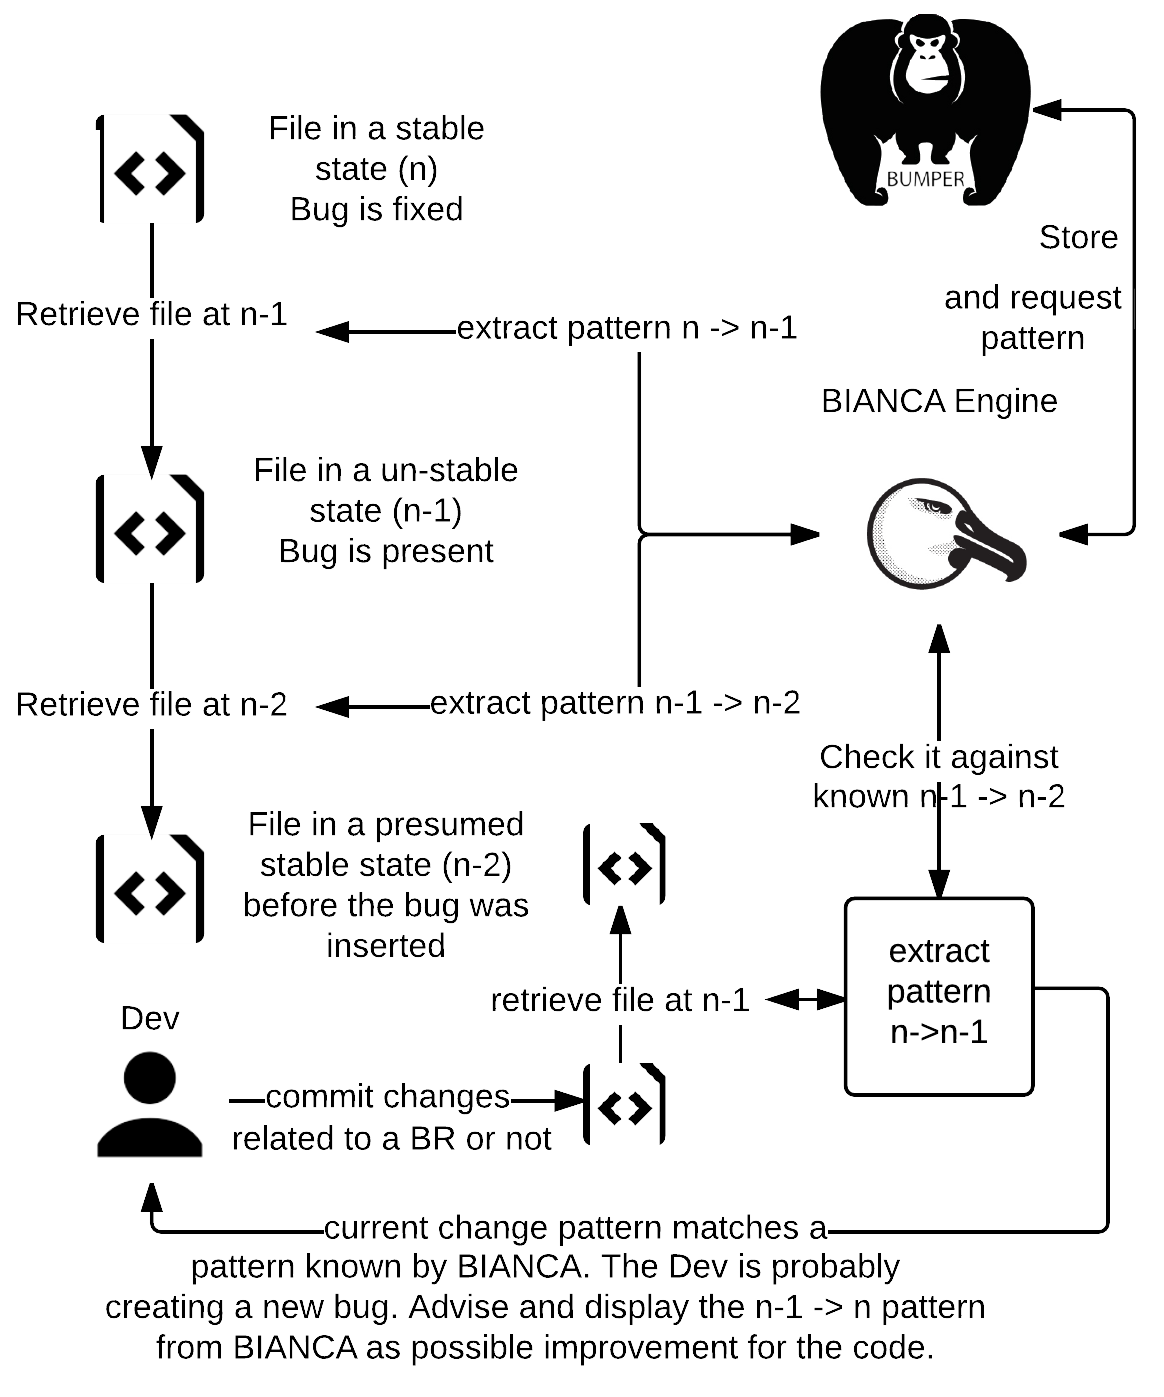
\includegraphics{media/bianca-approach.png}
    \caption{The BIANCA Approach
    \label{fig:bianca-approach}}
\end{figure}

{\tt BIANCA} builds a model where each issue is represented by three versions of the same file.
These three versions are stored in {\tt BUMPER}.
The first version $n$ is called the {\it stable state} because the code of this version was used to fix an issue.
The $n-1$ version, however, is called the {\it unstable state} as it was marked as containing an issue.
Finally, the third version is called the {\it before state} and represents the file before the introduction of the bug.
Hereafter, we refer to the {\it before state} as $n-2$.
{\tt BIANCA} extracts the change patterns form $n-2$ to $n-1$ and from $n-1$ to $n$.
It aslo generates the changes to go from $n-2$ to $n$.

When a developer commits new modifications, {\tt BIANCA} extracts the change pattern from the version $n_{dev}$ (current version) and $n-1_{dev}$ (version before modification) of the developer's source code and compare this change patterns to known $n-2$ to $n-1$ patterns.
If $n_{dev}$ to $n-1_{dev}$ matches a $n-2$ to $n-1$ then it means that the developer is inserting a known defect in the source code.
In such a case, {\tt BIANCA} will propose the related $n-1$ to $n$ pattern to the developer, so s/he could improve the source code and will show the related $n-2$ for the $n$ pattern so the developer will learn how to s/he should have modified the code in the first place.

Moreover, if the issue was previously reproduced by {\tt JCHARMING}, then {\tt BIANCA} will display the step to reproduce it.


To extract the change patterns and compare them, we used the same technique as the one presented in section \ref{sub:Extract and Save Blocks}.
The third and the fourth normalizations are removing all {\it less} important calls in the normalization one and two of {\tt RESEMBLE}.
We classify a call as less-important if, for example, it only does display-related functionalities such as generating HTML or printing something to the console. Finally, the fourth normalization will transform the code to an intermediate language of our own that will allow us to compare source code implemented in different programming languages.

Then, as in {\tt RESEMBLE}, if the LCS is above a user-defined threshold, then a warning is raised by {\tt BIANCA} alerting the developer that the commit is suspected to insert a defect.
The given defect is shown to the developer and can either force the commit if s/he don't find the warning relevant or abort the commit.

We believe that the warning, alongside the previously mined change patterns and steps to reproduce the suspected default --- provided by {\tt JCHARMING}, if available --- will statisfy developers in terms of actionable inteligence.
Thus, {\tt BIANCA} could succeed, where other tools failed, at being used in industrial environment	\cite{Lewis2013}.


\subsubsection{Early experiments}

We have experimented the efficiency of {\tt BIANCA} with the same datasets we used to build our bug taxonomy proposed in section \ref{chap:taxonomy}.

\begin{table}[h]
\begin{center}
\begin{tabular}{@{}c|c|c|c|c@{}}
\textbf{Dataset} & \textbf{Fixed Issues} & \textbf{Commit} & \textbf{Files} & \textbf{Projects} \\ \hline \hline
Netbeans         & 53,258          & 122,632     & 30,595         & 39                \\
Apache           & 49,449          & 106,366     & 38,111         & 349               \\
Total            & 102,707         & 229,153     & 68,809         & 388               \\ \hline \hline

\end{tabular}
\end{center}

\caption{Datasets\label{table:datasets-bianca}}
\end{table}

We choosed to use the same datasets for several reasons. First of all, we spare the time needed to collect new datasets. Then, because these datasets contain a very large system mainly implemented in Java: Netbeans; and 349 independent Apache projects implemented in a very wide range of programming language. Consequently, these datasets allow us to test the efficiency of our different code normalizations.

We ran two different experiments using the two first normalizations we described in section \ref{sec:bianca-approach}. Both experiments consider only a few months of history, from April to August 2008. While this could hinder the pertinence of our results, these five months of history contain 167,597 commits related to bug fix. Consequently, we believe our results to be representative.

The first experiment yields the result presented by Figure \ref{fig:bianca-exp-1}.

\begin{figure}[h!]
  \centering
    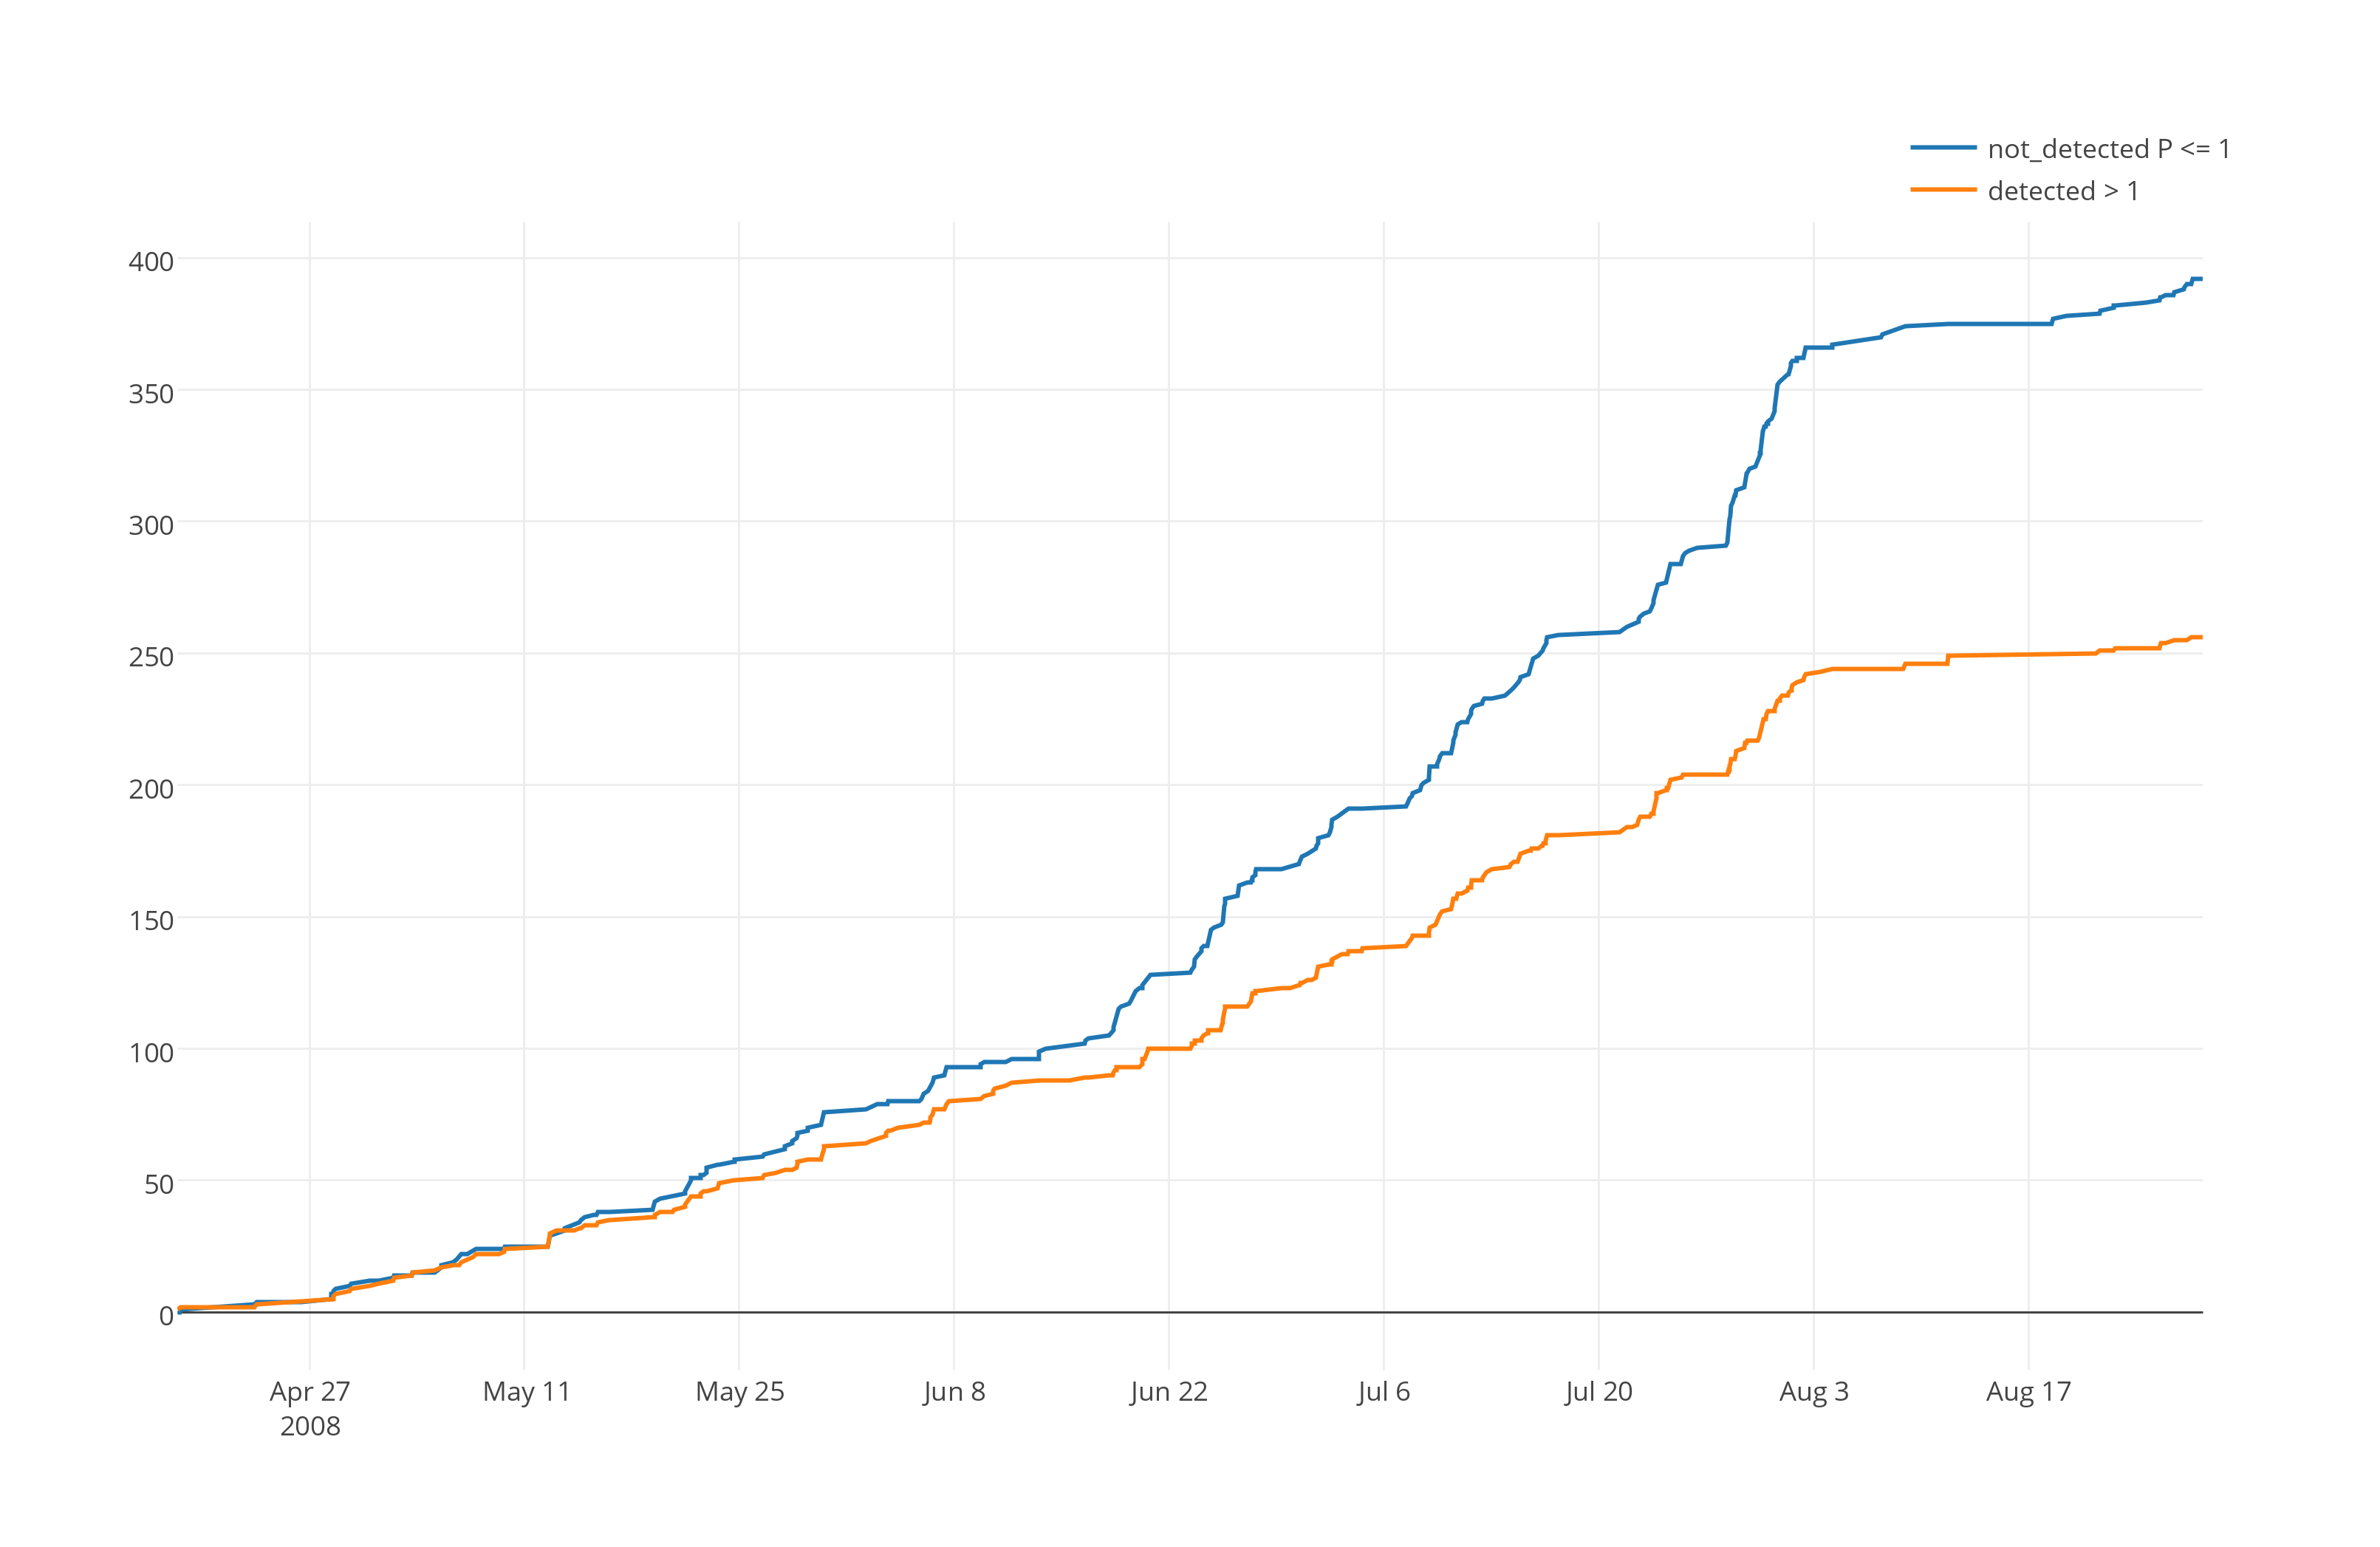
\includegraphics[scale=0.55]{media/bianca-13.png}
    \caption{{\tt BIANCA} warnings from April to August 2008 using the first normalization.
    \label{fig:bianca-exp-1}}
\end{figure}

With the first normalization, {\tt BIANCA} raised 69,519 warnings out of 167,597 (41.5\%) analyzed commits.
Out of these 69,519, 13.4\% turned out to be false positives. A false positive is a commit that have been tagged as introducing a bug by {\tt BIANCA} but did not according to the history.
However, false positives have to be dealt with carefully in this study as the commit might have introduced a bug but the bug could have not been reported yet.

In our second experiment, we used the second normalization and {\tt BIANCA} raised 83,627 warnings out of 167,597 (48.89\%) commit we analyze. However, the false positive rate increases to 21\%. Figure \ref{fig:bianca-exp-2} shows the results.

\begin{figure}[h!]
  \centering
    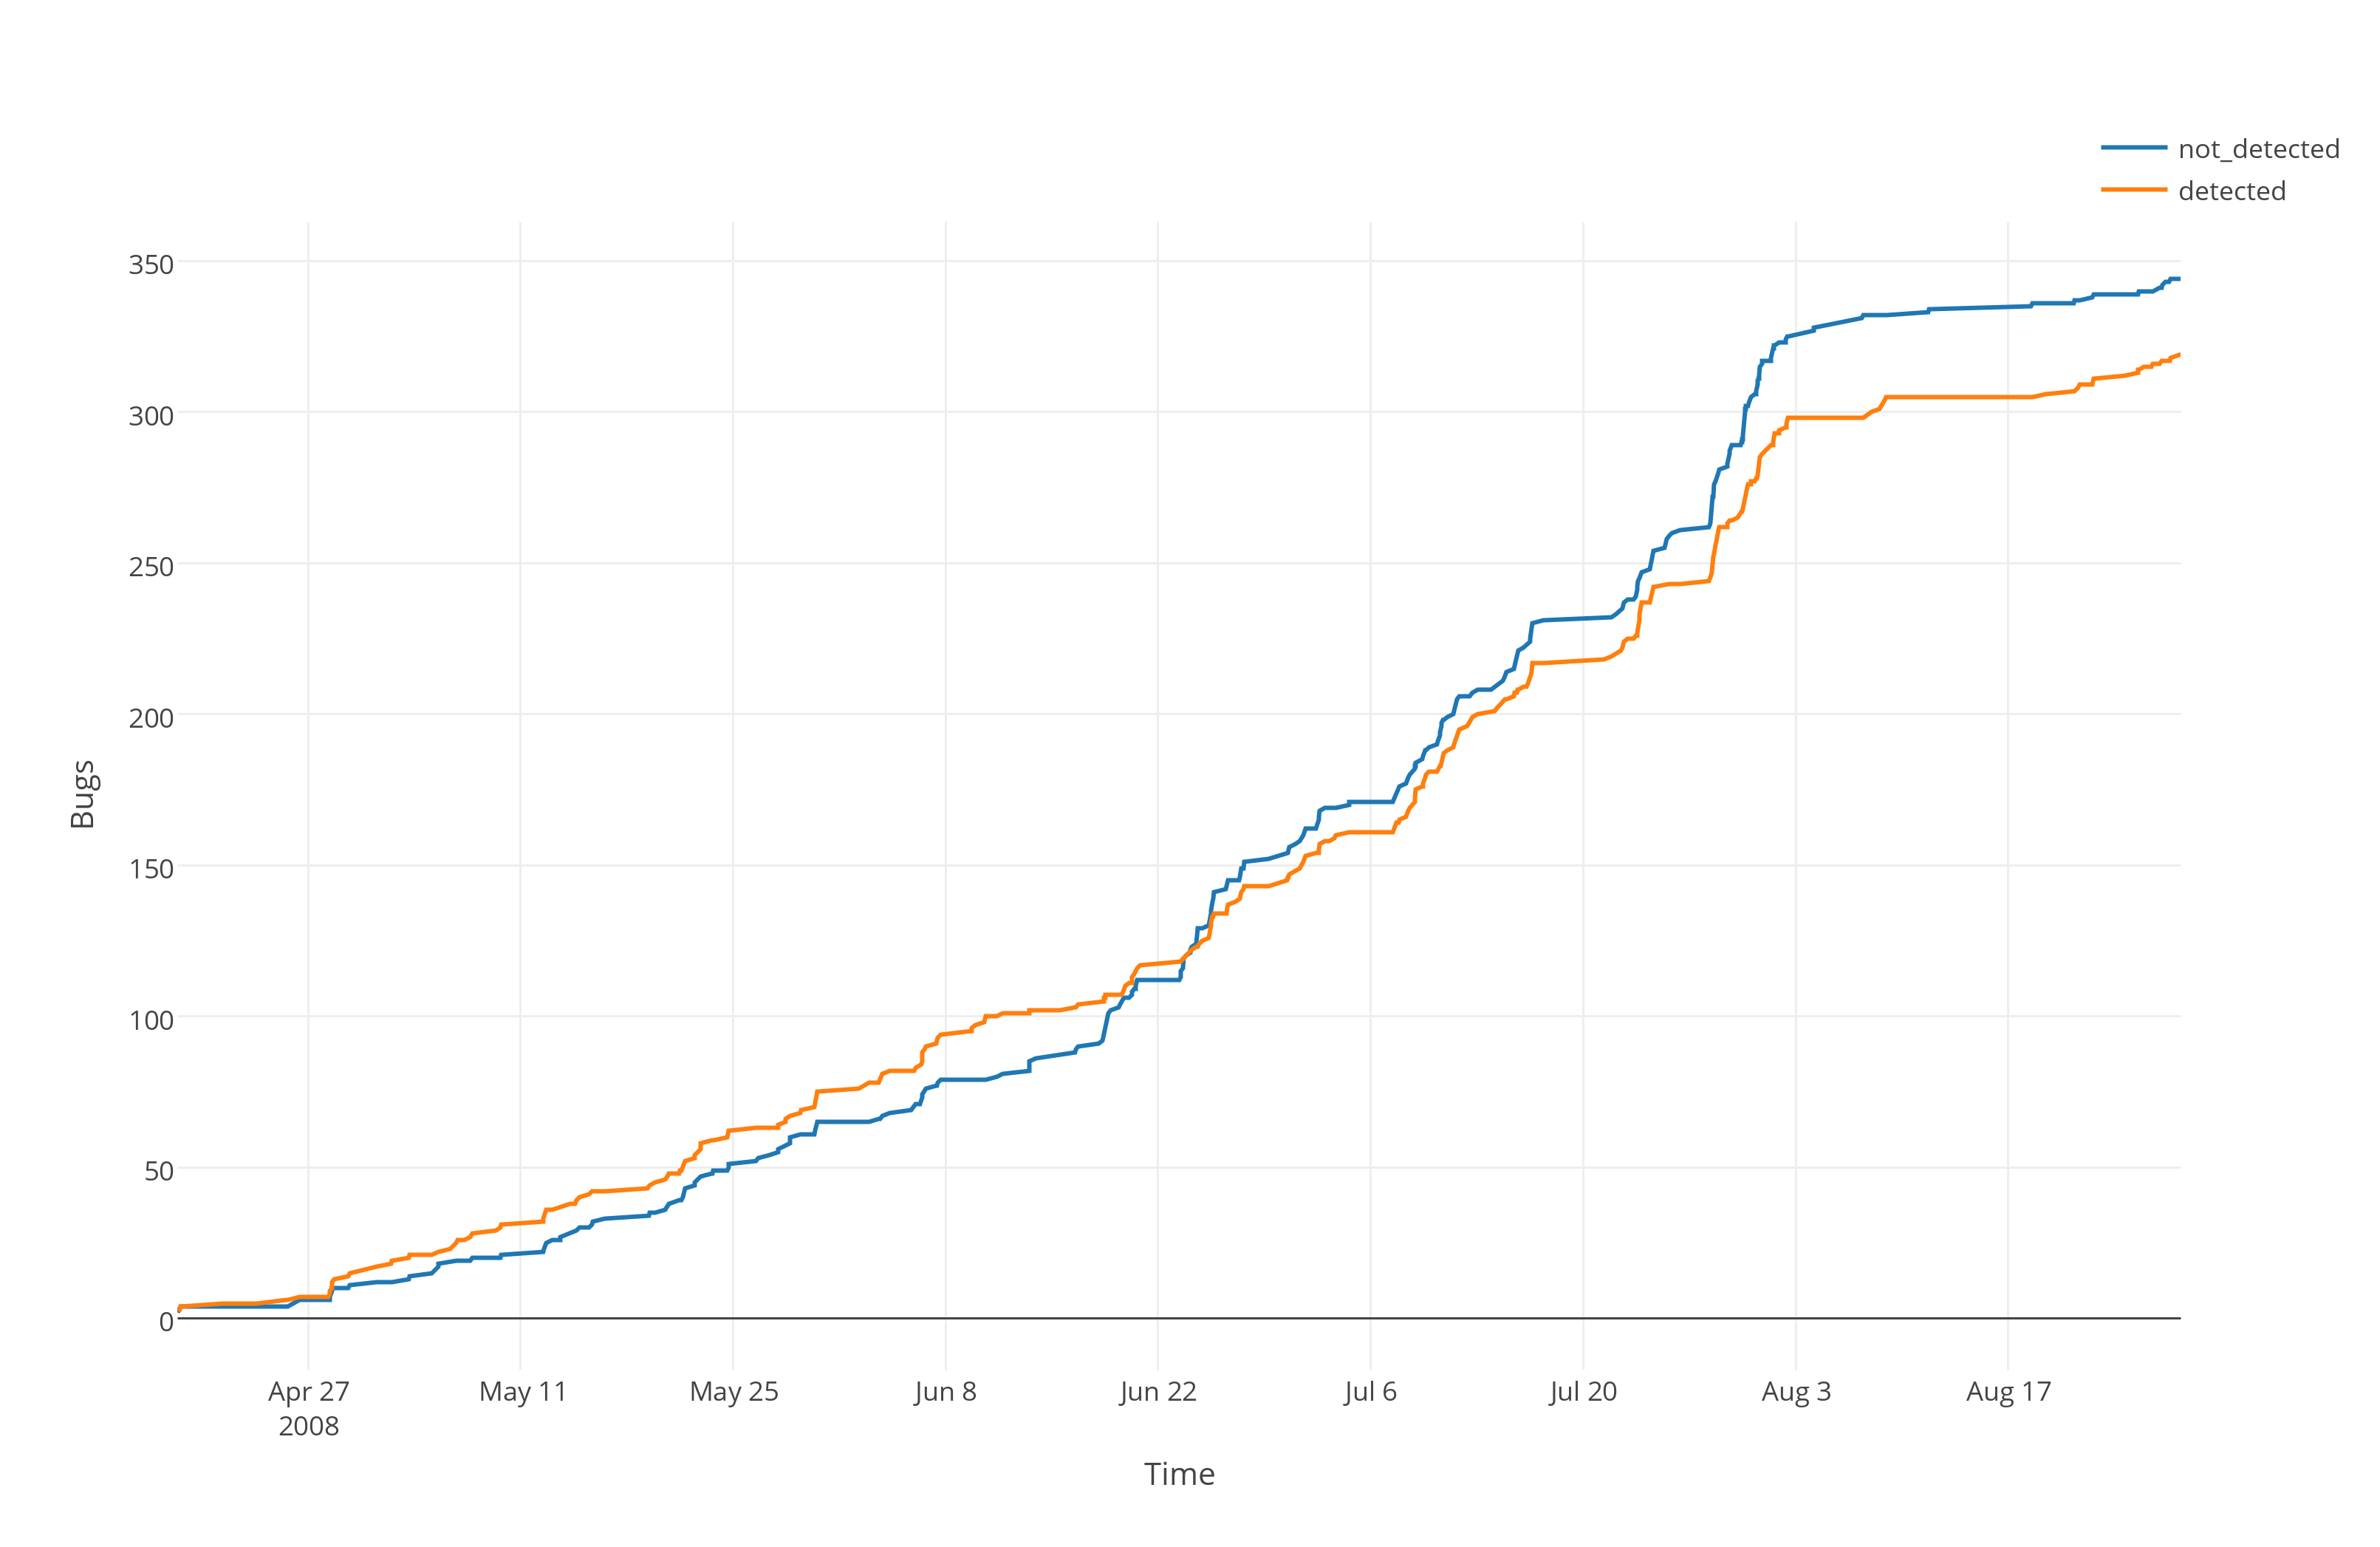
\includegraphics[scale=0.55]{media/bianca-20.png}
    \caption{{\tt BIANCA} warnings from April to August 2008 using the second normalization.
    \label{fig:bianca-exp-2}}
\end{figure}

{\tt BIANCA} experiments are still in their early stage and we are still trying to improve our normalizations in order to reduce the false positive rate.


%!TEX root = research_proposal.tex

\chapter{Remaining Work to Complete the Thesis\label{chap:plan}}

In this chapter, we summarize the state of the research and the work that needs to be completed in order to finalize the thesis.
We proceed according to the contributions listed on Section \ref{sec:objective-thesis}.


\section{An aggregate bug  repository for  developers  and  Researchers}

We introduced {\tt BUMPER} (BUg Metarepository for  dEvelopers  and  Researchers),  a  web-based  infrastructure
that  can  be  used  by  software  developers  and  researchers  to access  data  from  diverse  repositories  using  natural  language queries in a transparent manner, regardless of where the data was originally created and hosted.
{\tt BUMPER} have been showcased in the following publications:

\begin{itemize}
	\item Nayrolles, M. \& Hamou-Lhadj, W. BUMPER: A Tool to Cope with Natural Language Search of Millions Bugs and Fixes. In Proceeding of the International Conference on Software Analysis, Evolution, and Reengineering (SANER'16) - Tool Track, pages 649-652, 2016.
	\item Nayrolles, M. \& Hamou-Lhadj, W. BUMPER: Bug Metarepository Search Engine for Developers and Researchers. Consortium for Software Engineering Research Fall, 2015.
\end{itemize}

We consider this contribution to be 100\% complete.

\section{A bug reproduction technique based on a combination of crash traces and model checking.}

In this work, we proposed an approach, called {\tt JCHARMING} (Java CrasH Automatic Reproduction by directed Model checkING) that uses a combination of crash traces and model checking to automatically reproduce bugs that caused field failures.
{\tt JCHARMING} have been showcased in the following publications:

\begin{itemize}
	\item Nayrolles, M. , Hamou-Lhadj, W., Tahar, S. & Larsson, A. (2016). A Bug Reproduction Approach Based on Directed Model Checking and Crash Traces. Journal of Software: Evolution and Process. Wiley. 2016. (Accepted).
	\item Nayrolles, M. , Hamou-Lhadj, W., Tahar, S. & Larsson, A. JCHARMING : A Bug Reproduction Approach Using Crash Traces and Directed Model Checking. In Proceeding of the International Conference on Software Analysis, Evolution, and Reengineering (SANER'15), pages 101-110, 2015. (Best Paper Award).
\end{itemize}

We consider this contribution to be 100\% complete.

\section{An incremental approach for preventing bug and clone insertion at commit time}

We presented {\tt PRECCINT} (PREventing Clones INsertion at Commit Time), {\tt RESEMBLE} (REcommendation System based on cochangE Mining at Block LEvel) and {\tt BIANCA} (Bug Insertion ANticipation by Clone Analysis at merge time) in chapters \ref{chap:clone-detection-pragmatic} and \ref{chap:bianca}.

The efficiency of {\tt PRECCINT} have been accessed.
Early experiments have been conducted for {\tt BIANCA}.
However, we need to conduct additional experiments to measure the effiency {\tt RESEMBLE} and {\tt BIANCA}.

We consider this contribution to be 40\% complete.

\section{A new taxonomy of bugs based on the location of the correction --- an empirical Study}

We investigated the relationship between bugs by examining their locations of the fixes in chapter \ref{chap:taxonomy}.
We still need to refine our statistical analysis for our taxonomy.
More specifically, we need to compare each bug type one by one in addition to the comparison we have already done.

We consider this contribution to be 60\% complete.

\section{Publication Plan\label{sec:publication-plan}}

This section presents our planned publications over the course of the next years.

\begin{itemize}
	\item {\bf Publication 6}. {\tt PRECINCT} will be submitted to {\tt International Working Conference on Source Code Analysis and Manipulation, SCAM 2016}.
	\item {\bf Publication 7}. {\tt BIANCA} will be submitted to {\tt Journal of Software: Evolution and Process. 2016}.
	\item {\bf Publication 8}. {\tt RESEMBLE} will be submitted to {\tt International Conference Software Maintenance and Evolution, ICSME 2017}.
	\item {\bf Publication 9}. Our proposed bug taxonomy will be submitted to {\tt Empirical Software Engineering, ESE 2017}.
	\item {\bf Publication 10}. Our framework as a whole, {\tt BUMPER}, {\tt JCHARMING}, {\tt RESEMBLE} and {\tt BIANCA} will be submitted to {\tt Transaction of Software Engineering, TSE 2017}.
	\item {\bf Thesis}. In parallel to publications 9 and 10, I plan to write my Ph.D thesis.
\end{itemize}

Figure \ref{fig:planning} presents and overview of the publications planning and the relationship between the publications.

 \begin{figure}[h!]

 \centering
 \begin{ganttchart}
	  [
 inline
]{1}{30}
 \gantttitle{2014}{6}
 \gantttitle{2015}{6}
 \gantttitle{2016}{6}
 \gantttitle{2017}{6}
 \gantttitle{2018}{6}  \\
 \gantttitle{W}{2}
 \gantttitle{S}{2}
 \gantttitle{F}{2}
 \gantttitle{W}{2}
 \gantttitle{S}{2}
 \gantttitle{F}{2}
 \gantttitle{W}{2}
 \gantttitle{S}{2}
 \gantttitle{F}{2}
 \gantttitle{W}{2}
 \gantttitle{S}{2}
 \gantttitle{F}{2}
 \gantttitle{W}{2}
 \gantttitle{S}{2}
 \gantttitle{F}{2} \\


\ganttbar{$Courses$}{1}{4}

\\
\ganttbar{$JChar$}{5}{8}
\ganttbar{$JChar_2$}{12}{14}
\ganttbar{$Taxonomy$}{19}{22}
\\
\ganttbar{$Bumper$}{4}{11}
\ganttbar{$Pasmat$}{22}{25}
\\
\ganttbar{$Precinct$}{13}{16}
\\
\ganttbar{$Resemb$}{18}{20}
\ganttbar{$Thesis$}{25}{29}
\\
\ganttbar{$Bianca$}{15}{20}
\\


\ganttlink{elem0}{elem1}
\ganttlink{elem1}{elem2}
\ganttlink{elem2}{elem3}
\ganttlink{elem4}{elem2}
\ganttlink{elem4}{elem3}
\ganttlink{elem4}{elem6}
\ganttlink{elem6}{elem7}
\ganttlink{elem6}{elem9}

\ganttlink{elem6}{elem5}
\ganttlink{elem7}{elem5}
\ganttlink{elem9}{elem5}
\ganttlink{elem3}{elem5}
\ganttlink{elem5}{elem8}

 \end{ganttchart}


 \caption{Provisional Publication Planning\label{fig:planning}}
 \end{figure}

%!TEX root = research_proposal.tex

\chapter{Conclusion\label{chap:conclusion}}

The maintenance and evolution processes of system represent more than 70\% of the effort practioniers invest in them.
Hundreds of papers have been published with the aim to improve our knowledge of these processes in terms of issue triaging, issue prediction, duplicate issue detection, issue reproduction and co-changes prediction. 
All these publications gave meaning to the millions of issues that can be found in open source issue \& project and revision management systems. 
Context-aware IDE and think tank in open source architecure (\cite{chansler2011architecture}) open the path to approaches that support developpers during their programming sessions by levergaging past indexed knowledge and past architectures. 

In this research proposal, we first presented what are the most influencial papers in the different field our work lies on in Chapter \ref{chap:relwork}. 
Then, in chapter \ref{chap:thesis}, we identified current problems in the literature and our proposed solution to overcome them. 
Chapter \ref{chap:methodology} presented our proposal in details while chapter \ref{chap:plan} detailled our attempt planning.

More specifically, in Chapter \ref{chap:methodology}, we presented four approaches : {\tt BUMPER}, {\tt JCHARMING}, {\tt RESEMBLE}, {\tt BIANCA} we proposed a taxonomy of bugs. When combined into {\tt pErICOPE} \todo{Not sure yet about this name because of the Periscope app} (Ecosystem Improve source COde during Programming session with real-time mining of common knowlEdge), these tools (i) provide the possibility to search related software artifacts using natural language, (ii) accurately reproduce field-crash in lab environment, (iii) recommend improvement or completion of current block of code and (iv) prevent the introduction of clones / issues at commit time. 


{\tt BUMPER} has been designed to handle heavy traffic while {\tt JCHARMING} can reproduce 85\% of real-world issues we submitted to it. On its side {\tt BIANCA} is able to flag 41.5\% and 48.89\% of commit introducing bug as dangerous with 13.4\% and 21\% of false positive, respectively. 

Our future works, according to our publication plan described in section \ref{sec:publication-plan}, are as follows. First, we want to improve the performances of {\tt BIANCA} in terms of false positives. 
Then, create the IDE plugin that will support {\tt RESEMBLE}. Finally, we want to refined our taxonomy by including as many as datasets as possible.










% \section{Motivation}
%
% Architects, the ones that design buildings --- where mistakes cost lives --- spend at least five years at school and possibly their whole carriers to study, understand and reproduce great designs made by great architects.
% Software architects, however, begin in programing 101 by displaying the famous ``{\tt Hello World}'' statement and exponentially increase the complexity of their programs over their years of study and work.
% At some point, they will earn the title of software architect (or technical leader) because they have designed, maintained and evolved {\it enough} programs to be trustworthy on the matter.
% However, unlike building architects, they have to learn how to recognize, analyze and reproduce great architectural choices by themselves in addition of their day to day work.
% Of course, software developers do learn good practices such as design patterns \cite{Gamma2008} but in a very few occasions they will be presented with a state-of-the-art program built by great developers (Amy Brown {\it et al.} propose exactly that in their books \cite{chansler2011architecture, AmyBrown2012, Armstrong2013}).
%
% While this research is not about reforming how programming classes are taught, we still want to ease the access to this knowledge for developers during their programming sessions in order to ship better programs.
%
% In this research proposal, we shift the focus from merely mining revision and issue management system, where knowledge of great developers lies, to integrate them in their rightful place: as the keystone of software development and evolution activities.
% Extracting the ground truth from repositories helped engineers and practitioners to be better at building softwares as they know, for example, {\it how long it will take to fix a bug} \cite{Weiss2007}, {\it what makes a good bug report} \cite{Bettenburg2008} or {\it how to fix long-lived bugs} \cite{Saha2014}.
% Using these discoveries, tools can be created, on a per organization basis, to fit particular requirements such as programming languages, development processes or particular threshold. If we want to truthfully and deeply modify the software engineering landscape to have better softwares in terms of quality, maintainability and availability, we need to provide this information during the development, maintenance and evolution processes according to a specific context in an easy, reliable, actionable, free way.
%
% If we look back at the history of software engineering, the increase of processors' speed and decrease of their price allowed one to have a compiler on its own machine rather than sending one's code to the mainframe and receive compilation errors hours (days) later. This allowed, among other factors, the democratization of software engineering as {\it everyone}, belonging to a major organization or not, became able to build code. We believe that, it is now time to allow developers, engineering and practitioners, regardless of their programming language and contextual environment, not only to write and build code but to write and built qualitative, robust, resilient, easy to maintain and to fix code. What better way to do so than to {\it stand on the shoulder of giants} by having access to all the open sources repositories, including but not limited to, issues, tasks, bug fixes, patches, comments, good practices break down to the right level and provided at the right time during day to day programming sessions?
%
% What we concretely propose is an open-source, free, automatable tool suite that will allow everyone to (1) automatically reproduce field crashes in a controlled lab environment without any privacy concerns, (2) search in natural language the issues, comments, bugs, patches and fixes of tens of thousands of open source project, (3) prevent the insertion of defects in the source code during programming sessions by providing examples of the similar defect and how it has been fixed with a programming language abstraction. To support these tools we propose an empirical bug taxonomy (4).
%
%
%

\addcontentsline{toc}{chapter}{Bibliography}
\bibliography{library, russel}  %place your .bib files here
\bibliographystyle{alpha}                   %the bibliography style to use

\end{document}
